	\documentclass[aspectratio=43]{beamer}
\usepackage[latin1]{inputenc}
\usepackage{amsmath}
\usepackage{amsfonts}
\usepackage{amssymb}
\usepackage{makeidx}
\usepackage{graphicx}
\usepackage{array}

% Customization
\mode<presentation>{
	\usetheme{CambridgeUS}
	\usecolortheme{dolphin}
	\setbeamertemplate{navigation symbols}{}
}

% Define colors
\definecolor{darkgreen}{rgb}{0.0, 0.5, 0.13}
\definecolor{darkblue}{rgb}{0.0, 0.0, 0.55}
\definecolor{darkred}{rgb}{0.55, 0.0, 0.0}

% Title and author
\title[Higgs boson production at the LHC]{Higgs boson production at the LHC}
\author{\textbf {Jes\'us Urtasun Elizari}}
%\institute{\textbf {University of Milan}}
\date{Milan, February 2022}

\begin{document}

% Front slide
\begin{frame}

	%\maketitle
	\vspace{1.0 cm}
	
	\center{\color{blue}Higgs boson production at the Large Hadron Collider:\\
		accurate theoretical predictions at higher orders in QCD}
	
	\vspace{0.25 cm}
	\center{Jes\'us Urtasun Elizari}
	\center{PhD presentation - Milan, February 25th, 2022}

	\begin{figure}
		\minipage{1\textwidth}
		
\includegraphics[width = 3.0 cm]{plots/front_page/unimi.png}
		\hfill
		
\includegraphics[width = 3.0 cm]{plots/front_page/n3pdf.png}
		\hfill
		
\includegraphics[width = 3.0 cm]{plots/front_page/erc.png}
		\endminipage
	\end{figure}

	\vspace{1.0 cm}
	
	{\scriptsize \color{blue} This project has received funding from the European Union$'$s Horizon 2020 research and innovation program under grant agreement No 740006.}

\end{frame}

% Introduction
\begin{frame}

	\frametitle{Outline}
	
	\begin{enumerate}
		\item {\color{blue}Introduction to QCD}
		\begin{itemize}
			\item A historical approach
			\item Asymptotic freedom and pQCD
		\end{itemize}
		\item {\color{blue}QCD and collider physics}
		\begin{itemize}
			\item QCD Factorization
			\item Partonic cross section and perturbative QCD
		\end{itemize}
		\item {\color{blue}All order perturbative resummation}
		\begin{itemize}
			\item Higher order radiative corrections
			\item Resummation of large logarithmic corrections
			\item Resummed, asymptotic and fixed-order
		\end{itemize}
		\item {\color{blue}Precise and fast predictions for Higgs boson physics}
		\begin{itemize}
			\item Higgs production at the LHC
			\item HTurbo numerical code
			\item Preliminary results $\&$ Conclusions
		\end{itemize}
	\end{enumerate}
	
\end{frame}

%
% Introduction ...........................................................................
%

%
% Part 1 .................................................................................
% QCD and collider pysics ................................................................
%

% QCD and collider physics
\begin{frame}

	\center{\color{blue}Part I \\ QCD and collider physics}

\end{frame}

% QCD and the strong interactions
\begin{frame}

	\frametitle{Introduction}
	\framesubtitle{QCD and the strong interactions}
	
	\footnotesize
	
	\begin{itemize}
		\item QCD is the theory of the strong interactions
		\item Sector of the Standard describing fundamental interactions at the TeV scale
		\item Fundamental objects described as homogeneous field with quantum mechanical behavior U(1)$\times$SU(2)$\times$SU(3)
	\end{itemize}

\end{frame}

% QCD and the strong interactions
\begin{frame}

	\frametitle{Introduction}
	\framesubtitle{QCD and the strong interactions}
	
	\footnotesize
	
	How to explore proton's inner structure?

	\begin{figure}
		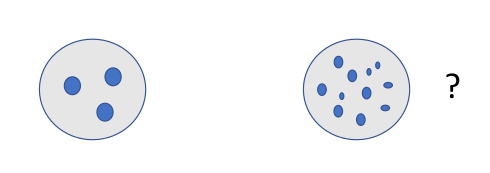
\includegraphics[width = 0.5\linewidth]{plots/part1/intro/protons.png}
	\end{figure}
	
	
	\begin{itemize}
		\item At different scales, hadrons show different behavior
		\item From point-like to complex internal dynamics
		\item Scattering experiments (DIS) and hadronic physics (LHC)
	\end{itemize}
	
	{\color{blue} \footnotesize "A way of describing high energy collisions is to consider any hadron as a composite object of point-like constituents $\longrightarrow$ \textbf{partons"} } R.Feynman, 1969 

\end{frame}

% Asymptotic freedom and pQCD
\begin{frame}

	\frametitle{QCD and collider physics}
	\framesubtitle{Asymptotic freedom and pQCD}

	\footnotesize
	
	\begin{columns}	
		
		\column{0.3\textwidth}
		
		\begin{figure}

			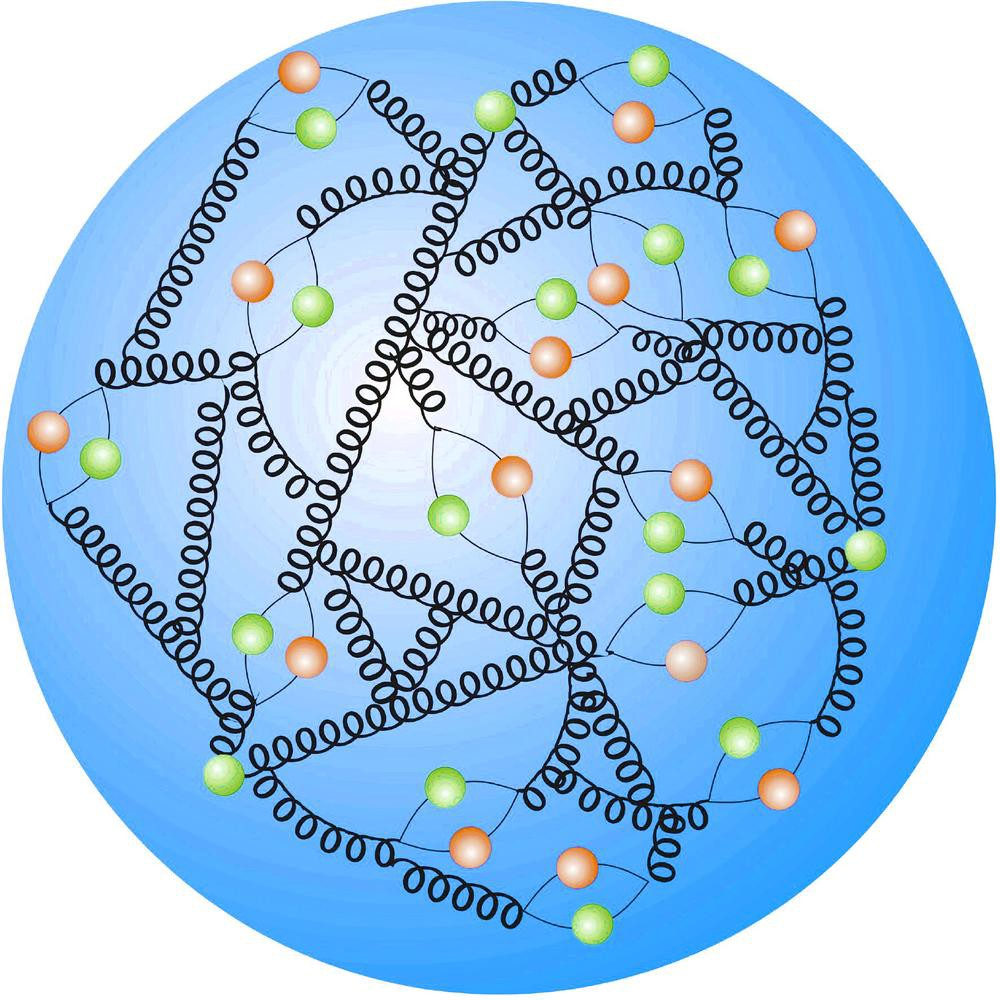
\includegraphics[width = 2 cm]{plots/part1/intro/proton2.jpg}
		\end{figure}
		
		\column{0.7\textwidth}
		
		\begin{itemize}
			\item Parton model as LO approximation to QCD
			\item Real QCD coupling strength changes with energy
			\item At high energies the hadron involves extremely complex internal dynamics
		\end{itemize}
		
	\end{columns}
	
	\vspace{1cm}
	\center \footnotesize QCD is strongly coupled at large scales / low energies $\longrightarrow$ confinement
	\center \footnotesize \color{red} Non-perturbative physics

\end{frame}

%Asymptotic freedom and pQCD
\begin{frame}
	
	\frametitle{QCD and collider physics}
	\framesubtitle{Asymptotic freedom and pQCD}
	
	\footnotesize
	
	\begin{itemize}
		\item Running coupling given by Renormalization Group Equation (RGE)
		\begin{equation}
		{\color{blue}\mu\frac{d\alpha_{s}(\mu)}{d\mu} = \beta(\alpha_{s}(\mu)) = -\sum_{n = 0}^{\infty} \beta_{n} \Big( \frac{\alpha_{s}}{\pi} \Big)^{n + 1}} \nonumber
		\end{equation}
		\item Coupling {\color{blue}$\alpha_{s}$} evolves with scale {\color{blue}$\mu$} as given by RGE $\rightarrow$ LO behavior driven by $\beta_{0}$
		\item $\beta_{0}^{\textrm{QED}} < 0 \implies$ strongly coupled at large energies, {\color{blue}UV divergent}
		\item $\beta_{0}^{\textrm{QCD}} > 0 \implies$ weakly coupled at large energies, {\color{red}IR divergent}
	\end{itemize}

\end{frame}

% Asymptotic freedom and pQCD
\begin{frame}

	\frametitle{QCD and collider physics}
	\framesubtitle{Asymptotic freedom and pQCD}
	
	\begin{columns}	
		
		\column{0.5\textwidth}
		
		\begin{figure}
			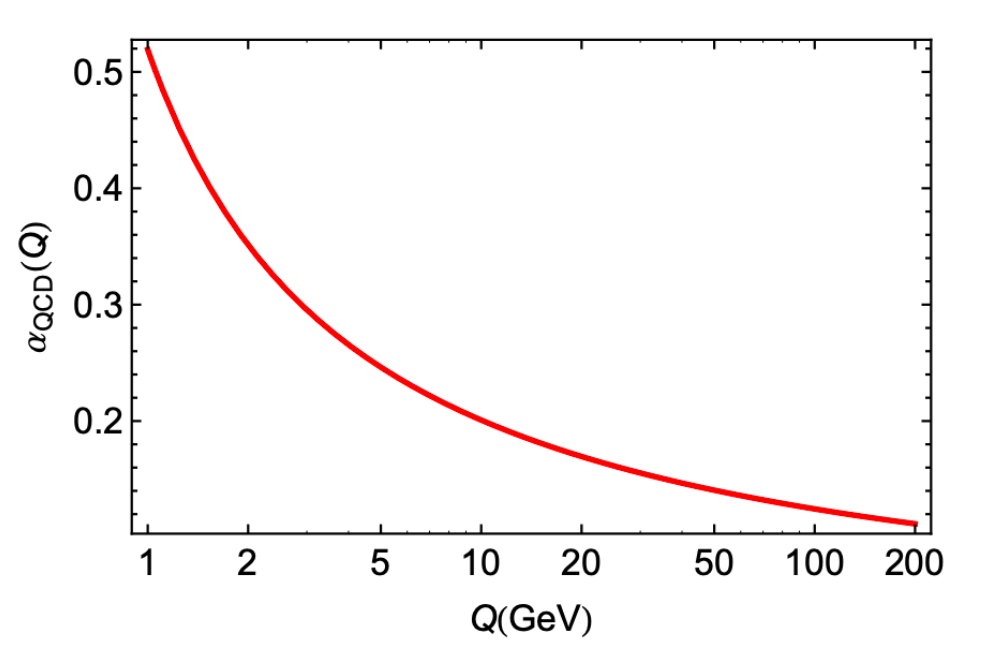
\includegraphics[width = 5 cm]{plots/part1/chapter1/qcd_running_coupling.png}
		\end{figure}
		
		\column{0.5\textwidth}
		
		\begin{itemize}
			\item \footnotesize Running coupling given by Renormalization Group Equation (RGE)
			\begin{equation}
			\alpha_{s}(\mu) = \frac{1}{\beta_{0} \log\big( \frac{\mu^{2}}{\Lambda_{\textrm{QCD}}^{2}}\big)} \nonumber
			\end{equation}
			\item \footnotesize $\beta_{0}$ LO of the $\beta$ function, is $ > 0$
			\item \footnotesize $\Lambda_{\textrm{QCD}}$, parameter that defines value of the coupling at large scales
		\end{itemize}
		
	\end{columns}
	
	\vspace{1cm}
	\center \footnotesize QCD is weakly coupled for $\mu >> \Lambda_{\textrm{QCD}} \longrightarrow$ asymptotically free
	\center \footnotesize \color{red} Perturbative Quantum Chromodynamics (pQCD)

\end{frame}

% Hadronic processes and factorization
\begin{frame}
	
	\frametitle{QCD and collider physics}
	\framesubtitle{Hadronic processes and factorization}
	
	\footnotesize
	
	\vspace{0.4 cm}
	
	\begin{figure}
		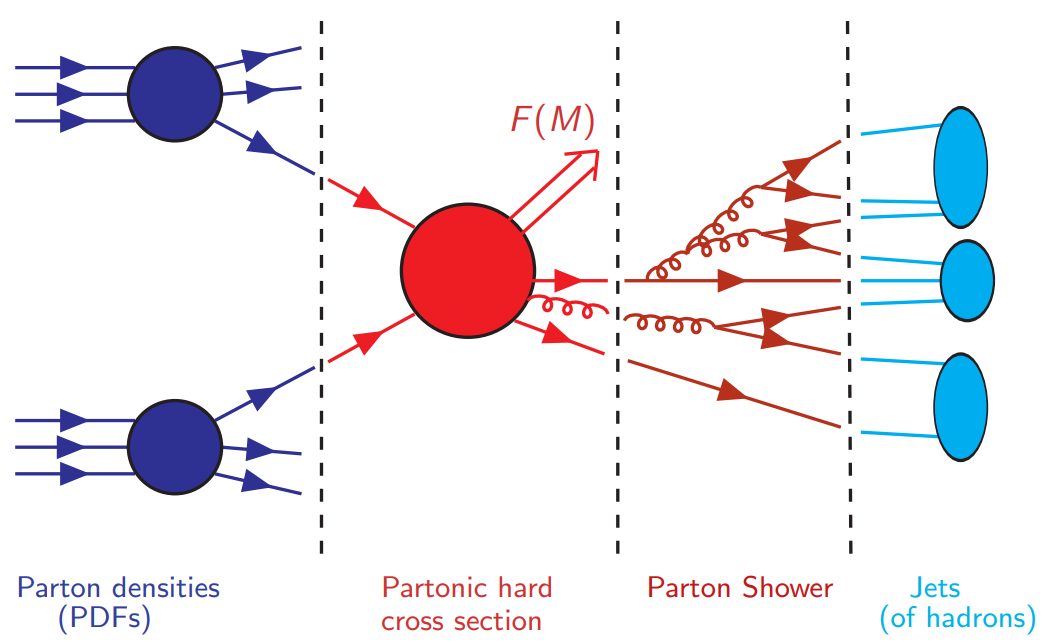
\includegraphics[width = 7 cm]{plots/part1/chapter2/factorization_1.png}
	\end{figure}
	
	\begin{itemize}
		\item LHC physic rely on hadronic collisions $\longrightarrow$ pQCD
		\item Compute cross section $\longrightarrow$ probability for a given process
	\end{itemize}

\end{frame}

% Hadronic processes and factorization
\begin{frame}

	\frametitle{QCD and collider physics}
	\framesubtitle{Hadronic processes and factorization}
	
	\footnotesize
	
	\vspace{0.4 cm}
	
	\begin{figure}
		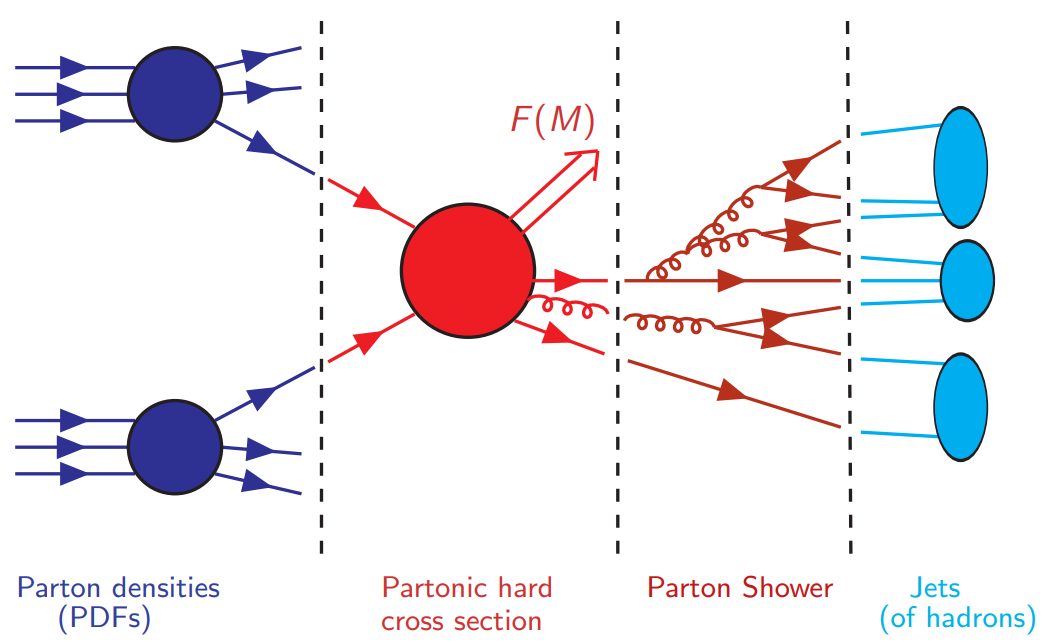
\includegraphics[width = 7 cm]{plots/part1/chapter2/factorization_1.png}
	\end{figure}
	
	Compute hadronic cross sections is a {\color{red}hard problem} $\longrightarrow$ {\color{blue} QCD Factorization}
	
	\begin{equation}
		\sigma^{\textrm{F}}(p_{1}, p_{2}) =
		\int_{0}^{1} dx_{1} dx_{2} \; {\color{blue} f_{\alpha}(x_{1}, \mu_{F}^{2}) \ast f_{\beta}(x_{2}, \mu_{F}^{2})}
		\; \ast \;  
		{\color{red}\hat{\sigma}^{\textrm{F}}_{\alpha \beta}(x_{1}p_{1}, x_{2}p_{2}, \alpha_{s}(\mu_{R}^{2}), \mu_{F}^{2})} \nonumber
	\end{equation}

\end{frame}

% Hadronic processes and factorization
\begin{frame}

	\frametitle{QCD and collider physics}
	\framesubtitle{Hadronic processes and factorization}
	
	\footnotesize
	
	\begin{figure}
		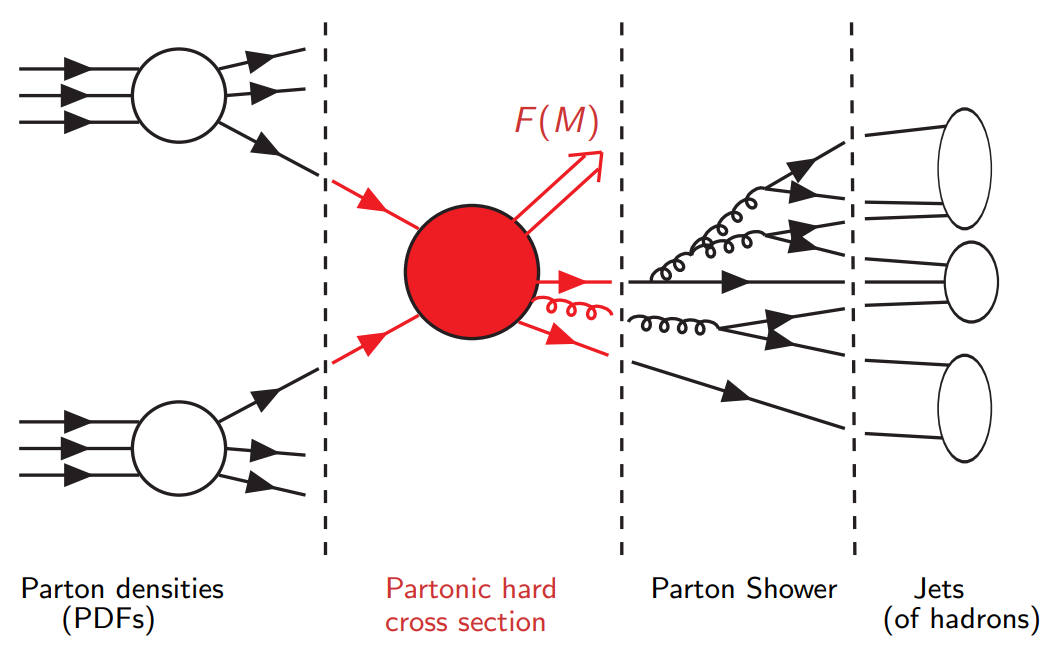
\includegraphics[width = 7 cm]{plots/part1/chapter2/factorization_2.png}
	\end{figure}
	
	\begin{itemize}
		\item Parton densities (PDFs) ${\color{blue} f_{\alpha}(x_{i}, \mu_{F}^{2})}$: non perturbative but universal
		\item Partonic cross section {\color{red}$\hat{\sigma}^{\textrm{F}}_{\alpha \beta}$}: process dependent but computable as perturbative series in $\alpha_{s}$
	\end{itemize}

\end{frame}

% Parton densities
\begin{frame}
	
	\frametitle{QCD and collider physics}
	\framesubtitle{Parton densities}
	
	\footnotesize

	\begin{columns}
	
	\column{0.5\textwidth}

	{\color{blue} Parton Distribution Functions: probability distribution of finding a particular parton \\ (u, d, ..., g) carrying a fraction x of the proton's momentum}

	\column{0.3\textwidth}
	
	\begin{figure}
		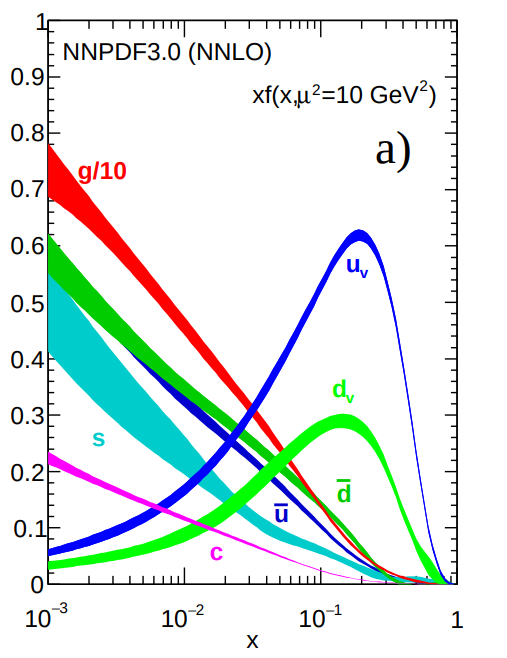
\includegraphics[width = 3 cm]{plots/part1/chapter2/PDF.png}
	\end{figure}
	
	\end{columns}

	\begin{itemize}
		\item Each parton has a different PDF $\longrightarrow$ ${\color{blue}u(x)}, {\color{green}d(x)}, ..., {\color{red}g(x)}$
		\item PDFs can not predicted and yet can not measured $\longrightarrow$ extracted from data \\ (MSTW, CTEQ, NNPDF collaborations)
		\item The N3PDF project: Machine Learning for PDFs determination \\
		{\color{blue}[Urtasun-Elizari et al.]} ref. at {\color{blue} \href{https://arxiv.org/abs/1910.07049}{1910.07049}}
	\end{itemize}

\end{frame}

% Partonic cross section and pQCD
\begin{frame}
	
	\frametitle{QCD and collider physics}
	\framesubtitle{Partonic cross section and pQCD}
	
	\footnotesize
	
	\begin{columns}
	
	\column{0.5\textwidth}
	
	\begin{itemize}
		\item Born cross section is the leading-order (LO) term of the perturbative series
		\item $\sigma^{(1)}, \sigma^{(2)}, \sigma^{(3)}$ are the NLO, NNLO, N$^{3}$LO corrections
	\end{itemize}
	
	\column{0.45\textwidth}
	
	\begin{figure}[!htb]
		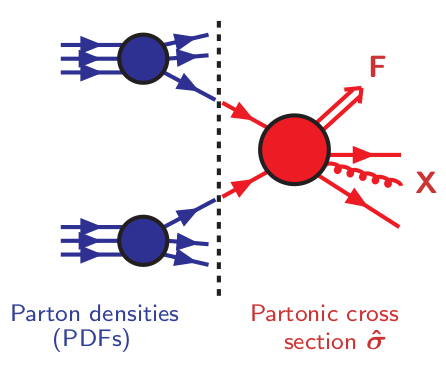
\includegraphics[width = 5 cm]{plots/part1/chapter2/factorization_3.png}
	\end{figure}
	
	\end{columns}
	
	\begin{equation}
		\hat{\sigma} = \sigma^{\texttt{Born}} \Big( 1 +
		\alpha_{s} \sigma^{(1)} + 
		\alpha_{s}^{2} \sigma^{(2)} + 
		\alpha_{s}^{3} \sigma^{(3)} + ... \Big) \nonumber
	\end{equation}
	
	\footnotesize Lower order predictions strongly depend on the auxiliary / unphysical scales \\ {\color{red}Need higher order corrections to increase theoretical accuracy!}

\end{frame}

% LHC physics
\begin{frame}
	
	\frametitle{QCD and collider physics}
	\framesubtitle{LHC phenomenology}
	
	\begin{figure}
		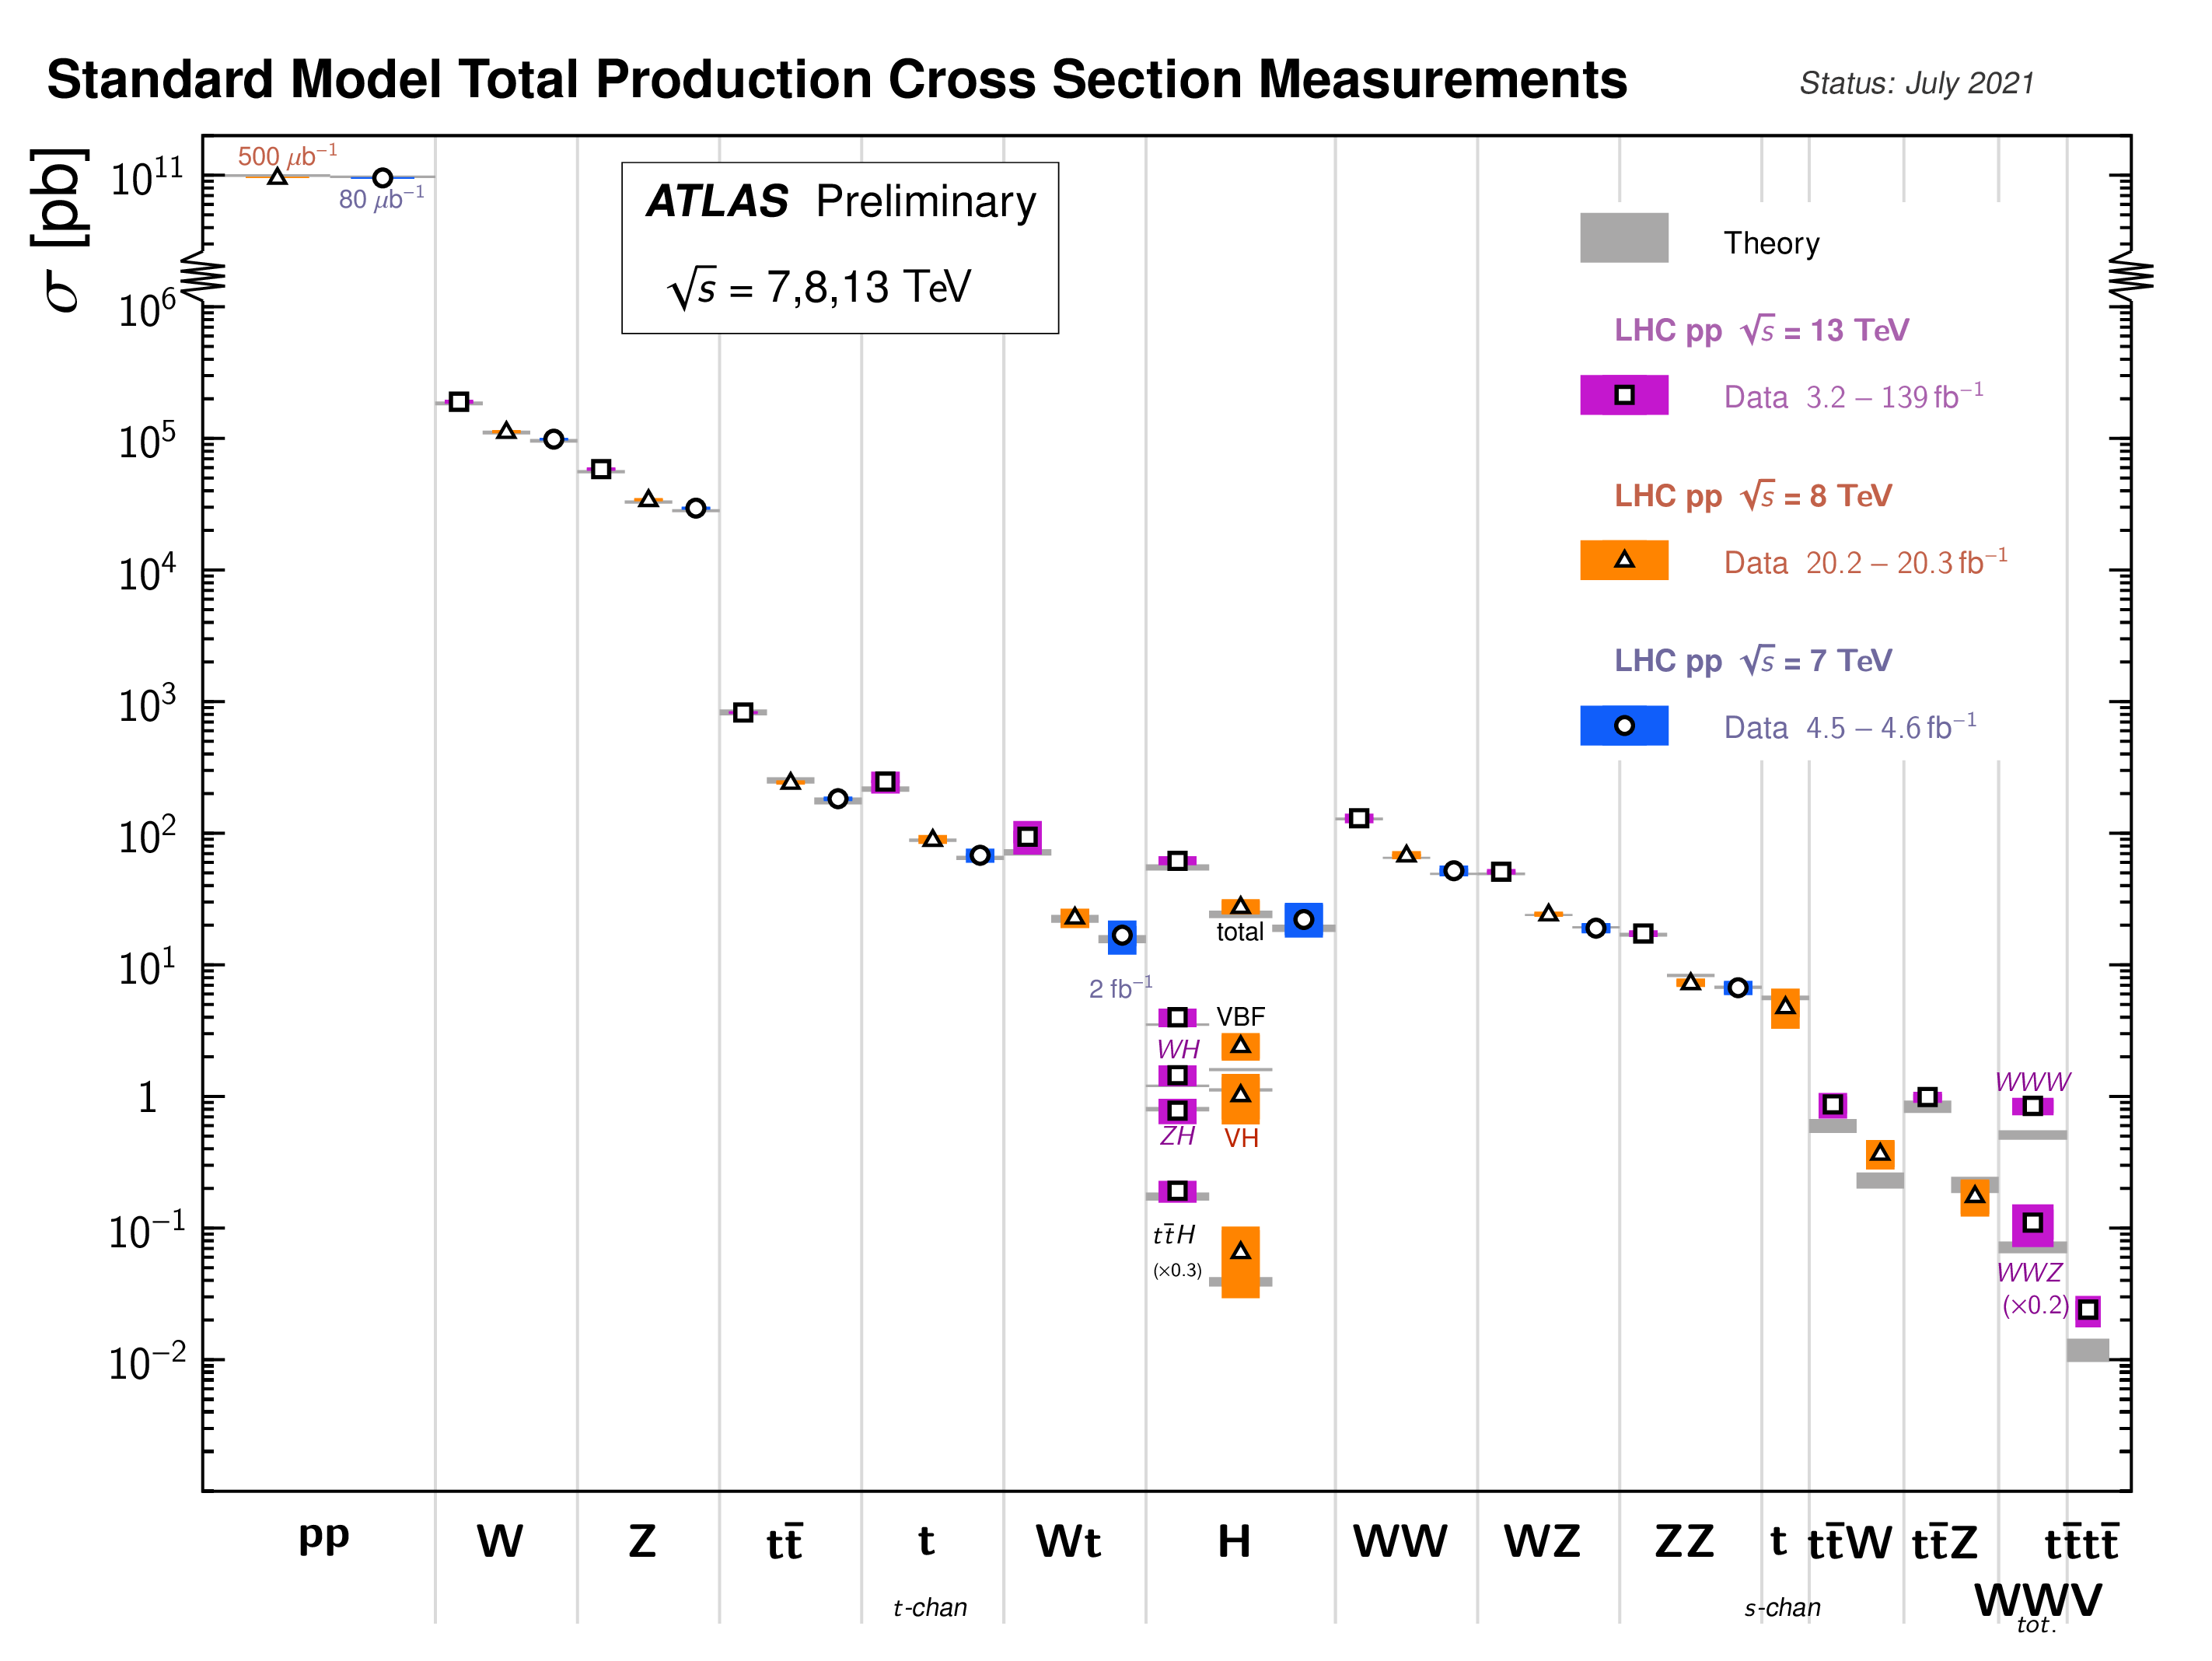
\includegraphics[width = 8.5 cm]{plots/part1/chapter3/lhc_measurements.png}
	\end{figure}

\end{frame}

% LHC physics
\begin{frame}
	
	\frametitle{QCD and collider physics}
	\framesubtitle{LHC phenomenology}
	
	\footnotesize
	
	Main processes studied in hadronic physics
	
	\begin{columns}
	
		\column{0.5\textwidth}
		
		\begin{itemize}
			\item Deep Inelastic Scattering (DIS)
			\item Drell-Yan lepton pair production
			\item Higgs boson production
		\end{itemize}
		
		\column{0.45\textwidth}
		
		\begin{figure}[!htb]
			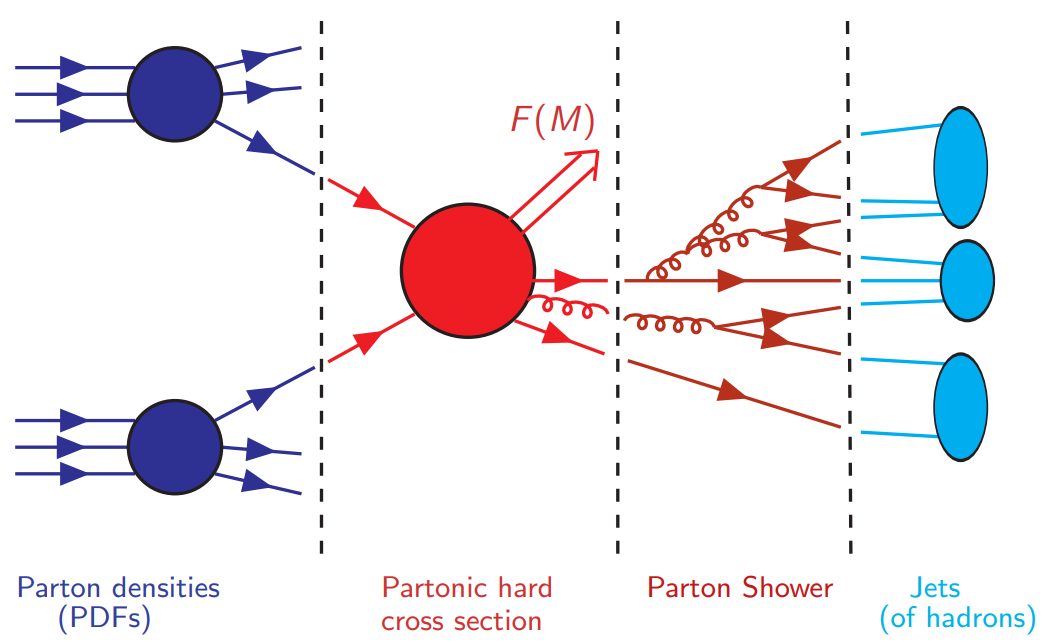
\includegraphics[width = 5 cm]{plots/part1/chapter2/factorization_1.png}
		\end{figure}
		
	\end{columns}

	\vspace{1 cm}
	
	\center Focus on Higgs production through gluon fusion
	
\end{frame}

%
% Part 2 .................................................................................
% All order resummation ..................................................................
%

% Dealing with divergences
\begin{frame}

	\center{\color{blue}Part II \\ All order resummation}

\end{frame}

% Higher order corrections
\begin{frame}

	\frametitle{Resummation in QCD}
	\framesubtitle{Higher order corrections - need for resummation}

	\footnotesize
	
	\begin{columns}
	
	\column{0.5\textwidth}
	
	\begin{enumerate}
		\item Calculation of higher order corrections is {\color{red}not an easy task} due to {\color{red} infrared (IR) soft and collinear singularities}
		\item Final state singularities {\color{blue}cancel} by combining real and virtual contributions $\longrightarrow$ KLN theorem
		\item Initial state collinear singularities {\color{blue}factorized} inside the PDFs
	\end{enumerate}
	
	\column{0.45\textwidth}
	\begin{figure}[!htb]
		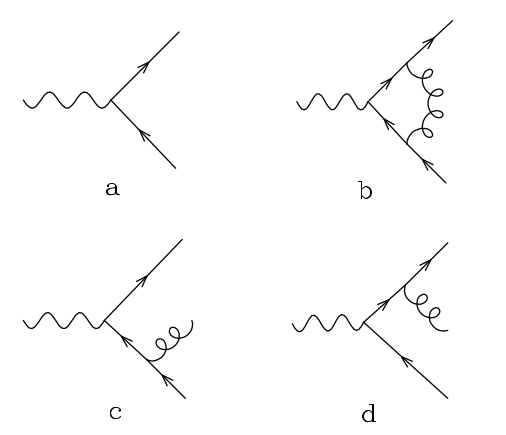
\includegraphics[width = \linewidth]{plots/part2/qcd_corrections.png}
	\end{figure}
	
	\end{columns}

	\vspace{0.5 cm}
	
	Cancellation only works in completely inclusive final states!

\end{frame}

% qT resummation I
\begin{frame}

	\frametitle{Resummation in QCD}
	\framesubtitle{$q_{\perp}$ resummation}
	
	\footnotesize
	
	\begin{columns}
	
		\column{0.55\textwidth}
		
		\begin{itemize}
			\item Describing exclusive final states \\
			\item Study the differential $q_{\perp}$ distribution \\
			$h_{1}(p_{1}) + h_{2}(p_{2}) \longrightarrow F(M, {\color{red}q_{\perp}}) + X$
		\end{itemize}
		
		\column{0.45\textwidth}
		
		\begin{figure}
			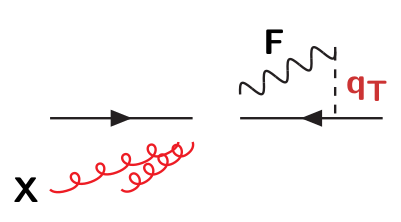
\includegraphics[width = 4cm]{plots/part2/qT_diagram.png}
		\end{figure}

	\end{columns}
 
	$\int_{0}^{Q_{\perp}^{2}} \; dq_{\perp}^{2} \frac{d\hat{\sigma}}{dq_{\perp}^{2}} \sim c_{0} + \alpha_{s}(c_{12}L^{2} + c_{11}L + c_{10}) + ..., \textrm{\quad where \quad} L = \ln (M^{2} / q_{\perp}^{2})$

	\begin{figure}
		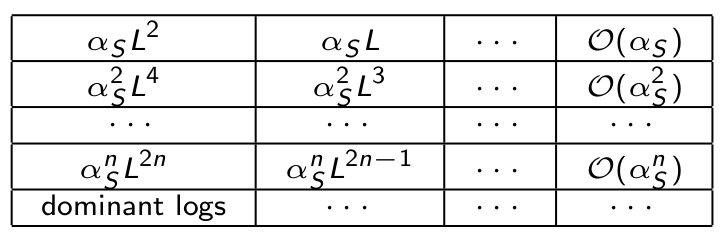
\includegraphics[width = 7cm]{plots/part2/qT_logs_table.png}
	\end{figure}

	Truncated fixed-order predictions $\rightarrow$ {\color{red}enhanced $\alpha_{s}^{n}\ln^{m}(M^{2}/q_{\perp}^{2})$ appear}

\end{frame}

% Resummation in QCD II
\begin{frame}

	\frametitle{Resummation in QCD}
	\framesubtitle{$q_{\perp}$ resummation}

	\footnotesize Separate partonic $q_{\perp}$ distribution as follows
	
	\begin{equation}
		\frac{d\hat{\sigma}_{ab}}{dq_{\perp}^{2}} =
		\Bigg[ \frac{d\hat{\sigma}^{\textrm{(res.)}}_{ab}}{dq_{\perp}^{2}} \Bigg]_{\textrm{l.a.}} + 
		\Bigg[ \frac{d\hat{\sigma}^{\textrm{(fin.)}}_{ab}}{dq_{\perp}^{2}} \Bigg]_{\textrm{f.o.}} \textrm{\quad, \quad such that} \nonumber
	\end{equation}

	\begin{align}
		\int_{0}^{q_{\perp}^{2}} dq_{\perp}^{2} \frac{d\hat{\sigma}^{\textrm{(res.)}}_{ab}}{dq_{\perp}^{2}} \sim & \sum \alpha_{s}^{n} \log^{m} \bigg( \frac{M^{2}}{q_{\perp}^{2}} \bigg) \textrm{\quad for \quad} q_{\perp} \rightarrow 0 \nonumber \\
		\lim_{q_{\perp} \rightarrow 0}\int_{0}^{q_{\perp}^{2}} dq_{\perp}^{2} \frac{d\hat{\sigma}^{\textrm{(fin.)}}_{ab}}{dq_{\perp}^{2}} &= 0 \nonumber 
	\end{align}

	\footnotesize Resummed and finite components can be matched (LL+LO, NLL+NLO,\\ NNLO+NNLL, ...) to have uniform accuracy in a wide range of $q_{\perp}$
\end{frame}

% qT resummation III
\begin{frame}

	\frametitle{Resummation in QCD}
	\framesubtitle{Resummed component}
	
	\footnotesize
	
	Resummation holds in impact parameter space $b$
	
	\begin{equation}
		\frac{d\hat{\sigma}_{ab}^{\textrm{(res.)}}}{dq_{\perp}^{2}} = \frac{M^{2}}{\hat{s}} \int db \; \frac{b}{2} \; J_{0}(b q_{\perp}) \; {\color{red} \mathcal{W}_{ab}(b, M)} \nonumber
	\end{equation}
	 
	with ${\color{red}\mathcal{W}_{ab}}$ also expressed in Mellin space (with respect to $z = M^{2}/\hat{s}$)
	\begin{equation}
		{\color{red} \mathcal{W}_{N}(b, M) = \mathcal{H}_{N}(\alpha_{s}) \times \exp\{\mathcal{G}_{N}(\alpha_{s}, L)\}} \quad\textrm{being}\quad L \equiv \log(M^{2}b^{2}) \nonumber
	\end{equation}

	\begin{itemize}
		\item Large logarithms exponentiated in the universal Sudakov form factor {\color{red}$\mathcal{G}_{N}(\alpha_{s}, L)$}
		\item Constant (b-independent) terms factorized in the process dependent hard factor {\color{red}$\mathcal{H}_{N}(\alpha_{s})$}
	\end{itemize}
	
\end{frame}

% qT resummation IV
\begin{frame}
	
	\frametitle{Resummation in QCD}
	\framesubtitle{Resummed component}
	
	\footnotesize
	
	Sudakov factor $\mathcal{G}_{N}$ and hard coefficient $\mathcal{H}_{N}$ can be expanded as perturbative series in $\alpha_{s}$
	\begin{align}
	\mathcal{G}_{N}(\alpha_{s}, L) &= L\;g^{(1)}(\alpha_{s}L) + g^{(2)}(\alpha_{s}L) + \frac{\alpha_{s}}{\pi}g^{(3)}(\alpha_{s}L) + ... \nonumber \\
	\mathcal{H}_{N}(\alpha_{s}) &= 1 + \alpha_{s}\mathcal{H}^{(1)} + \alpha_{s}^{2}\mathcal{H}^{(2)} + ...  \nonumber
	\end{align}
	
	For each new order implement a factor of $\mathcal{G}_{N}$ and Hard $\mathcal{H}_{N}$
	
	\begin{columns}
		
		\column{0.45\textwidth}
		
		\begin{align}
		&\textrm{LL} (\sim \alpha_{s}^{n}L^{n+1}): g^{(1)}, \hat{\sigma}^{(0)} \nonumber \\
		&\textrm{NLL} (\sim \alpha_{s}^{n}L^{n}): g^{(2)}, \mathcal{H}^{(1)} \nonumber \\
		&\textrm{NNLL} (\sim \alpha_{s}^{n}L^{n-1}): g^{(3)}, \mathcal{H}^{(2)} \nonumber
		\end{align}
		
		\column{0.45\textwidth}
		
		Each term $g^{(i)}$ and $\mathcal{H}^{(i)}$ in the series becomes increasingly complicated \\
		\vspace{0.25 cm}
		Current codes able to produce only up to NNLL predictions!
		
	\end{columns}

\end{frame}

% qT resummation III
\begin{frame}
	
	\frametitle{Resummation in QCD}
	\framesubtitle{Finite component}
	
	\footnotesize
	
	Finite component by fixed-order truncation of the resummed cross section
	
	\begin{equation}
		\frac{d\hat{\sigma}^{\textrm{(fin.)}}_{ab}}{dq_{\perp}^{2}} =
		\Bigg[ \frac{d\hat{\sigma}_{ab}}{dq_{\perp}^{2}} \Bigg]_{\textrm{f.o.}} + 
		\Bigg[ \frac{d\hat{\sigma}^{\textrm{(res.)}}_{ab}}{dq_{\perp}^{2}} \Bigg]_{\textrm{f.o.}} \nonumber
	\end{equation}
	
	the truncation of the resummed cross section is written in terms of the $\Sigma$ coefficients
	
	\begin{equation}
		{\color{red} \mathcal{W}_{a, b}(b, M) = \sigma^{(0)} \times \mathcal{H}_{N}(\alpha_{s}) \times \alpha_{s}^{n} \Sigma^{n}(z, L)} \quad\textrm{being}\quad L \equiv \log(M^{2}b^{2}) \nonumber
	\end{equation}

\end{frame}

%
% Part 3 .................................................................................
% HTurbo numerical implementation ........................................................
%

% Part 3
\begin{frame}

	\center{\color{blue}Part III \\ HTurbo numerical implementation}

\end{frame}

% Resummation for Higgs differential distribution
\begin{frame}
	
	\frametitle{HTurbo}
	\framesubtitle{Resummation for Higgs differential distribution}

	\footnotesize
	
	\begin{itemize}
		\item Fast and accurate predictions for Higgs boson production cross section
		\item Predictions for differential cross section $d\sigma^{\textrm{H}} / dq_{\perp}^{2}$
		\item Numerical implementation of resummed and finite components
	\end{itemize}

	\begin{columns}
		
		\column{0.5\textwidth}
		
		\begin{equation}
			d\sigma^{\textrm{H}}_{\textrm{(N)NLL+(N)LO}} = 
			d\sigma^{\textrm{(res.)}}_{\textrm{(N)NLL}} - 
			d\sigma^{\textrm{(asy.)}}_{\textrm{(N)LO}} + 
			d\sigma^{\textrm{(f.o.)}}_{\textrm{(N)LO}} \; , \nonumber
		\end{equation}
	
		\begin{align}
			d\sigma^{\textrm{(res.)}}_{\textrm{(N)NLL}} &= \hat{\sigma}^{\textrm{H}}_{\textrm{LO}} \times \mathcal{H}_{\textrm{(N)LO}} \times \exp{\mathcal{G}}_{\textrm{(N)NLL}} \; , \nonumber \\
			d\sigma^{\textrm{(asy.)}}_{\textrm{(N)LO}} &= \hat{\sigma}^{\textrm{H}}_{\textrm{LO}} \times \Sigma_{\textrm{(N)LO}} \; ,\nonumber
		\end{align}
	
		\column{0.45\textwidth}
		
		\begin{figure}
			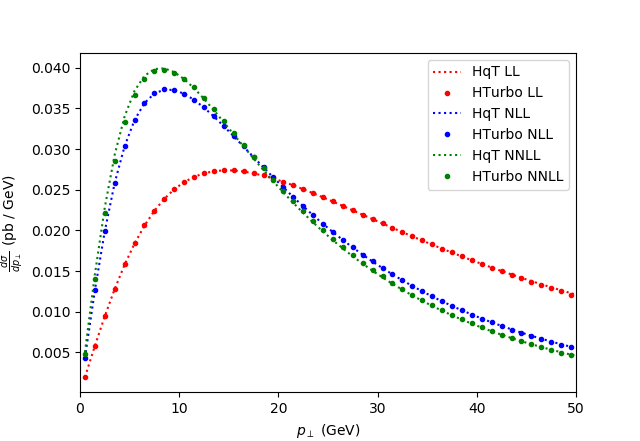
\includegraphics[width = 5 cm]{plots/part3/chapter6/higgs_qt_all.png}
		\end{figure}	
		
	\end{columns}

\end{frame}

% HqT and HRes
\begin{frame}

	\frametitle{HTurbo}
	\framesubtitle{Predictions for Higgs $q_{\perp}$ distribution}
	
	\footnotesize
	
	\begin{columns}
		
		\column{0.5\textwidth}
			
		\begin{itemize}
			\item $q_{\perp}$ resummation implemented in numerical codes \textbf{HRes}, \textbf{HRes}, \textbf{HNNLO} {\color{blue}[Catani, de Florian, Ferrera, Grazzini, Tommasini]} 
			\item Higher order accuracy require \\
			{\color{red}high computation times}
			\item NNLL predictions can take up to 48h $\longrightarrow$ need for {\color{red} fast numerical implementations}
		\end{itemize}

		\column{0.45\textwidth}
	
		\begin{figure}
			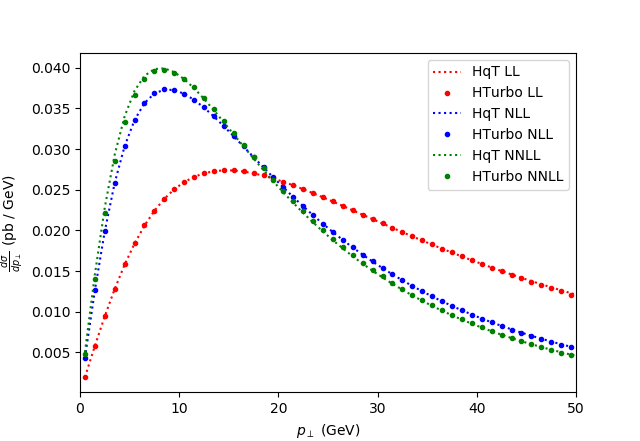
\includegraphics[width = 6 cm]{plots/part3/chapter6/higgs_qt_all.png}
		\end{figure}		
			
	\end{columns}

	\vspace{0.5 cm}
	
	Codes producing fast and accurate predictions are needed for precision era of the LHC
	
\end{frame}

% DYturbo I
\begin{frame}

	\frametitle{HTurbo}
	\framesubtitle{Starting point: DYTurbo}

	\footnotesize
	
	Numerical code \textbf{DYTurbo} {\color{blue}[Camarda et al.]} ref. at {\color{blue} \href{https://arxiv.org/abs/1910.07049}{1910.07049}}, fast and precise $q_{\perp}$ resummation and several improvements for Drell-Yan ($h_{1}h_{2} \rightarrow V + X \rightarrow l^{+}l^{-} + X$) 
	
	\vspace{0.5 cm}
	
	{\color{red}First goal}: set up a numerical code for Higgs boson production starting from  \textbf{DYTurbo}
 
	\begin{itemize}
		\item Set LO amplitude $gg \rightarrow H$
		\item Set Sudakov and Hard coefficients for resummed component
		\item Set $\Sigma$ coefficients for asymptotic term
		\item Implement MC producing the LO and NLO H+jet cross sections
		\item Compare with \textbf{HRes} and \textbf{HqT}
	\end{itemize}

	\vspace{0.2 cm}

	{\color{red}Final goal}: extend theoretical accuracy up to N$^{3}$LL+N$^{3}$LO

\end{frame}

% DYturbo II
\begin{frame}

	\frametitle{HTurbo}
	\framesubtitle{Implementation of Higgs boson factors}

	\footnotesize
	
	Sudakov factor $\mathcal{G}_{N}$ and hard coefficient $\mathcal{H}_{N}$ can be expanded as perturbative series in $\alpha_{s}$
	\begin{align}
		\mathcal{G}_{N}(\alpha_{s}, L) &= L\;g^{(1)}(\alpha_{s}L) + g^{(2)}(\alpha_{s}L) + \frac{\alpha_{s}}{\pi}g^{(3)}(\alpha_{s}L) + ... \nonumber \\
		\mathcal{H}_{N}(\alpha_{s}) &= 1 + \alpha_{s}\mathcal{H}^{(1)} + \alpha_{s}^{2}\mathcal{H}^{(2)} + ...  \nonumber
	\end{align}
	
	For each new order implement a factor of $\mathcal{G}_{N}$ and Hard $\mathcal{H}_{N}$
	
	\begin{columns}
		
		\column{0.45\textwidth}

		\begin{align}
			&\textrm{LL} (\sim \alpha_{s}^{n}L^{n+1}): g^{(1)}, \hat{\sigma}^{(0)} \nonumber \\
			&\textrm{NLL} (\sim \alpha_{s}^{n}L^{n}): g^{(2)}, \mathcal{H}^{(1)} \nonumber \\
			&\textrm{NNLL} (\sim \alpha_{s}^{n}L^{n-1}): g^{(3)}, \mathcal{H}^{(2)} \nonumber
		\end{align}
	
		\column{0.45\textwidth}
		
		Start by building predictions up to NNLO+NNLL, then add {\color{blue}N$^{3}$LO+N$^{3}$LL}
		
	\end{columns}

\end{frame}

% DYturbo II
\begin{frame}

	\frametitle{HTurbo}
	\framesubtitle{Code optimization}
	
	\footnotesize
	
	Optimized reimplementation of \textbf{HqT}, \textbf{HRes} and \textbf{HNNLO} for $q_{T}$-resummation
	
	\vspace{0.2 cm}
		
	\begin{itemize}
		\item \textbf{C++} structure with \textbf{Fortran} interfaces $\rightarrow$ Multi-threading
		\item Optimization in the integration routines / integral transforms 
		\begin{itemize}
			\item Factorize boson and decay kinematics
			\item Gauss-Legendre quadrature rules (1-dim.)
			\item Vegas/Cuhre through \textbf{Cuba} (multi-dim.)
		\end{itemize}
	\end{itemize}
	
	\vspace{0.5cm}
	
	Comparison \textbf{HRes} and \textbf{HTurbo} - speed performance \\
	
	\center
	\begin{tabular}{ | c | c | c | }
		\hline
		Predictions & \textbf{HRes} & \textbf{HTurbo} \\ 
		\hline
		resummed NNLL & 10h & 10' \\
		\hline
		combined NNLO+NNLL & 48h & 2h \\
		\hline
	\end{tabular}

	
\end{frame}

% Results - Benchmark HRes - NLL resummed
\begin{frame}
	
	\frametitle{Results}
	\framesubtitle{Comparison HTurbo and HRes - NLL resummed}
	
	\footnotesize
	
	\begin{columns}
		
		\column{0.5\textwidth}
		
		\begin{figure}
			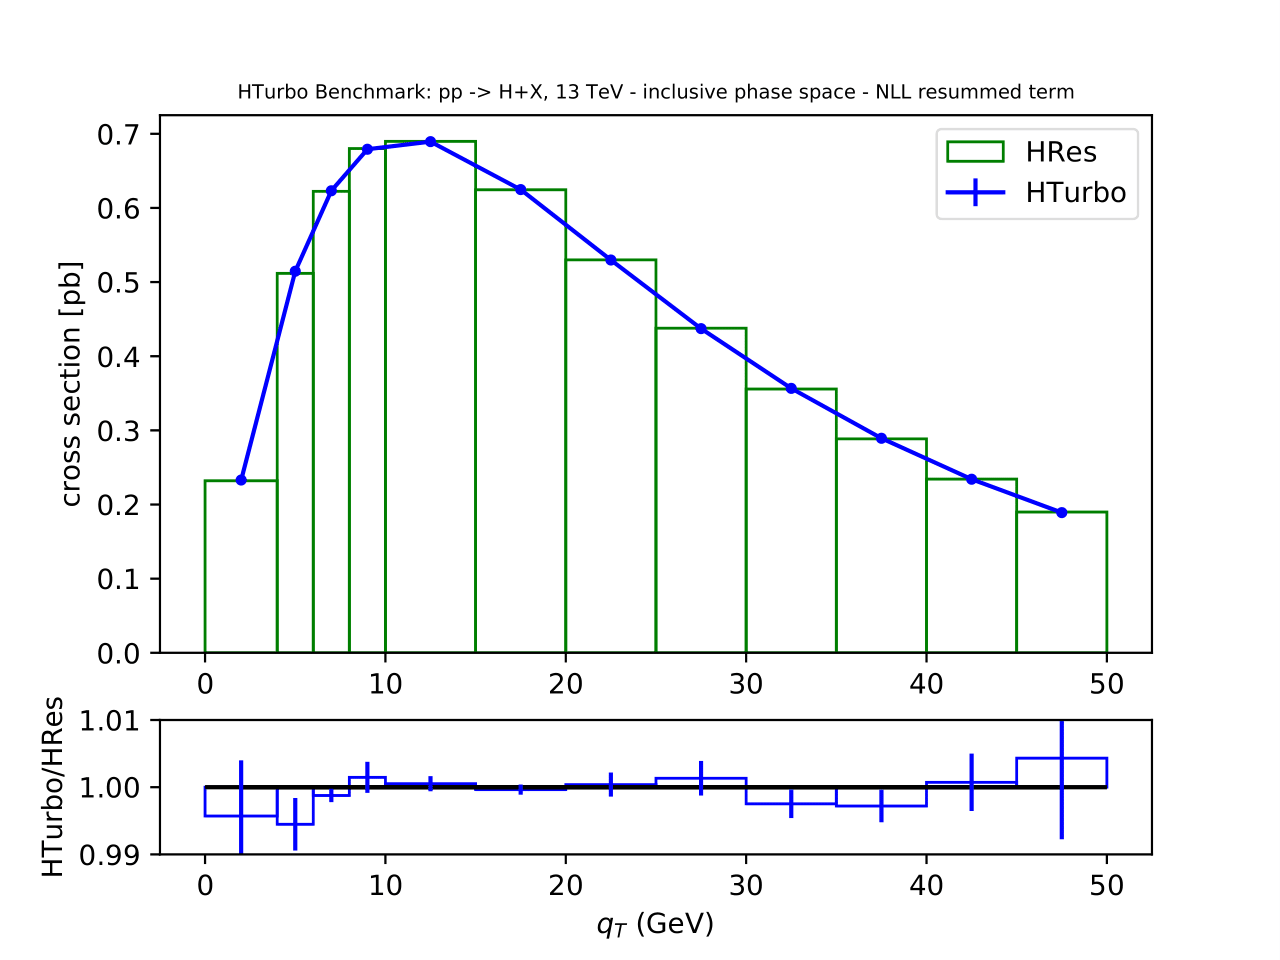
\includegraphics[width = 7cm]{plots/part3/chapter6/nlo-res-1.png}
		\end{figure}
		
		\column{0.5\textwidth}
		
		\begin{figure}
			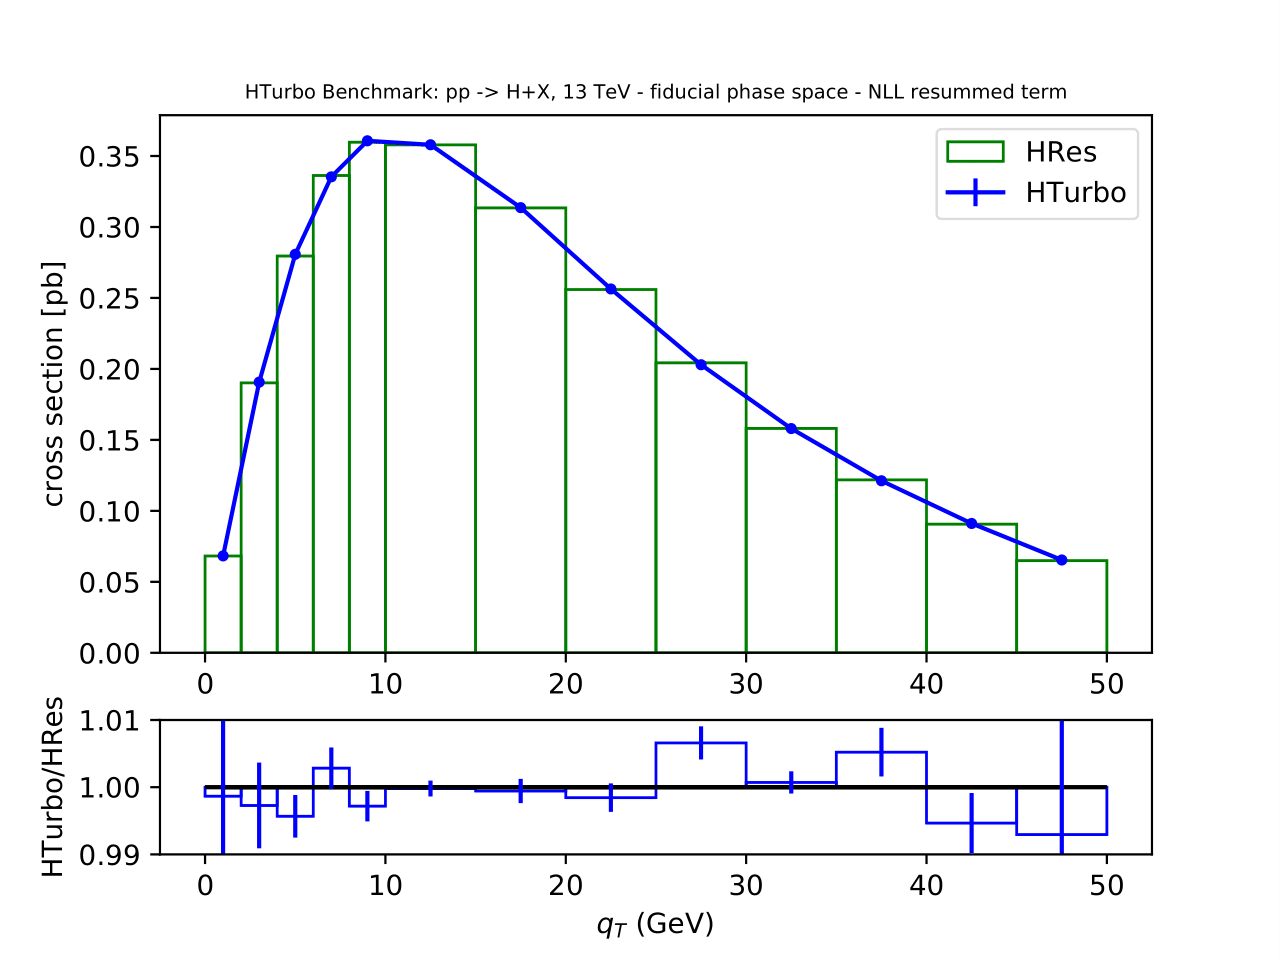
\includegraphics[width = 7cm]{plots/part3/chapter6/nlo-res-fid-1.png}
		\end{figure}
		
	\end{columns}
	
	\begin{itemize}
		\item Cross section for fully inclusive (LHS) and fiducial (RHS) phase space {\color{darkgreen}$\checkmark$} 
		\item CM energy $\sqrt s = 13$ GeV and PDF set \texttt{NNPDF31\_nlo\_as\_0118 PDF} set
	\end{itemize}

\end{frame}

% Results - Benchmark HRes - NNLL resummed
\begin{frame}
	
	\frametitle{Results}
	\framesubtitle{Comparison HTurbo and HRes - NNLL resummed}
	
	\footnotesize
	
	\begin{columns}
	
	\column{0.5\textwidth}
	
	\begin{figure}
		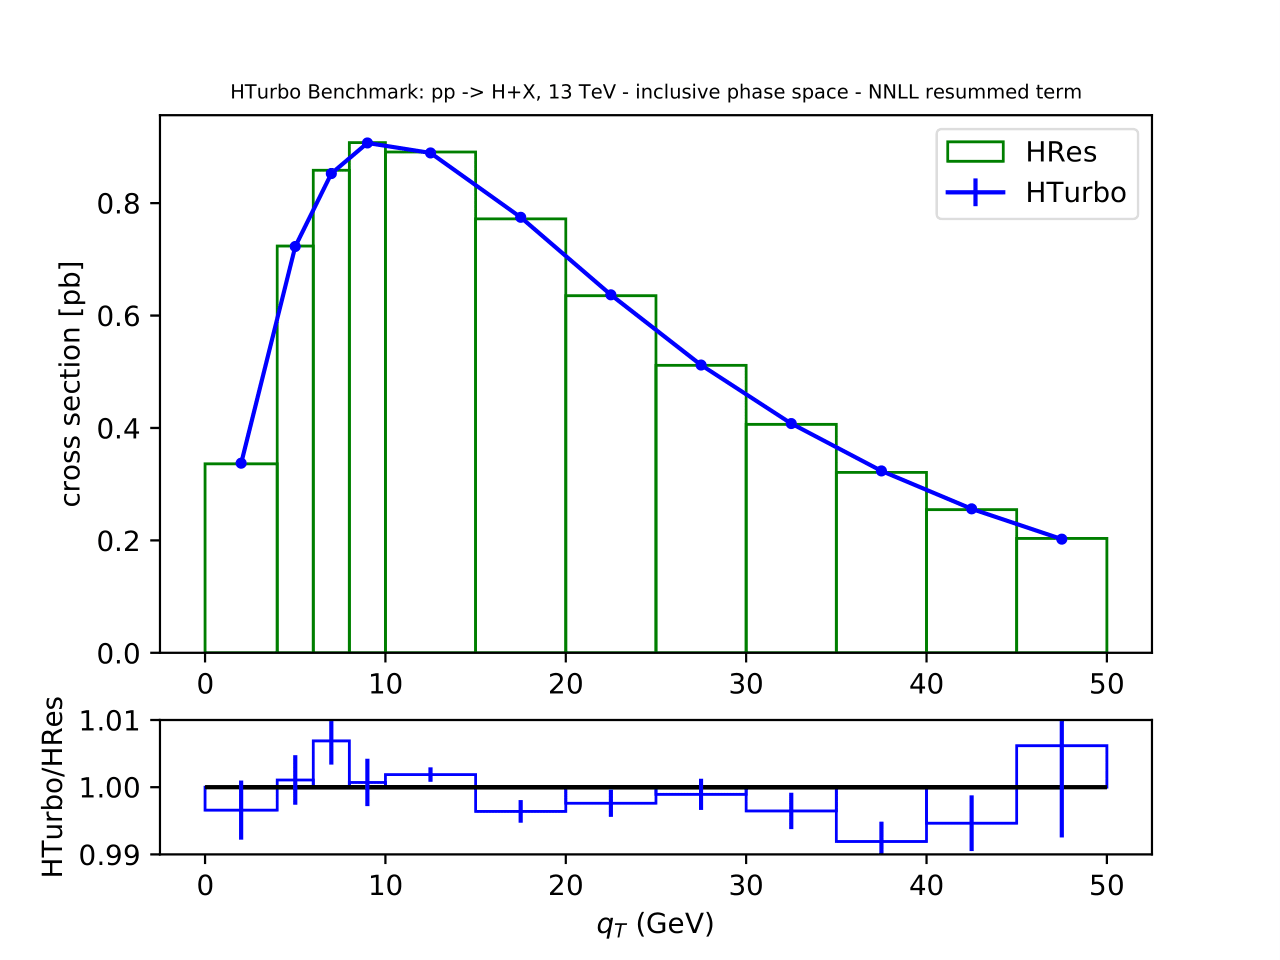
\includegraphics[width = 7cm]{plots/part3/chapter6/nnlo-res-1.png}
	\end{figure}
	
	\column{0.5\textwidth}
	
	\begin{figure}
		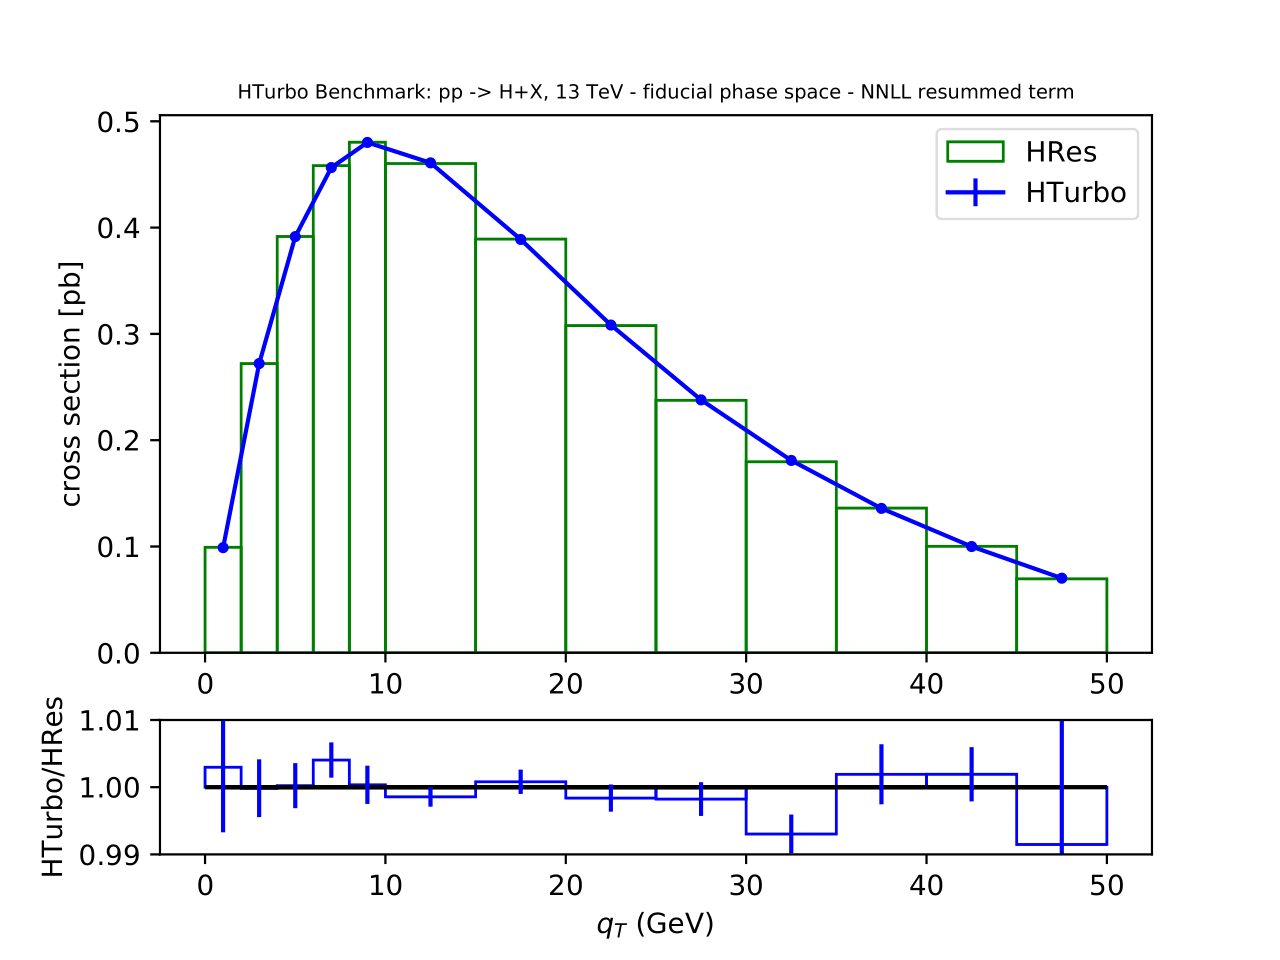
\includegraphics[width = 7cm]{plots/part3/chapter6/nnlo-res-fid-1.png}
	\end{figure}
	
	\end{columns}
	
	\begin{itemize}
	\item Cross section for fully inclusive (LHS) and fiducial (RHS) phase space {\color{darkgreen}$\checkmark$} 
	\item CM energy $\sqrt s = 13$ GeV and PDF set \texttt{NNPDF31\_nnlo\_as\_0118 PDF} set
	\end{itemize}

\end{frame}

% Results - Benchmark HRes - LO asymptotic
\begin{frame}
	
	\frametitle{Results}
	\framesubtitle{Comparison HTurbo and HRes - LO asymptotic}
	
	\footnotesize
	
	\begin{columns}
		
		\column{0.5\textwidth}
		
		\begin{figure}
			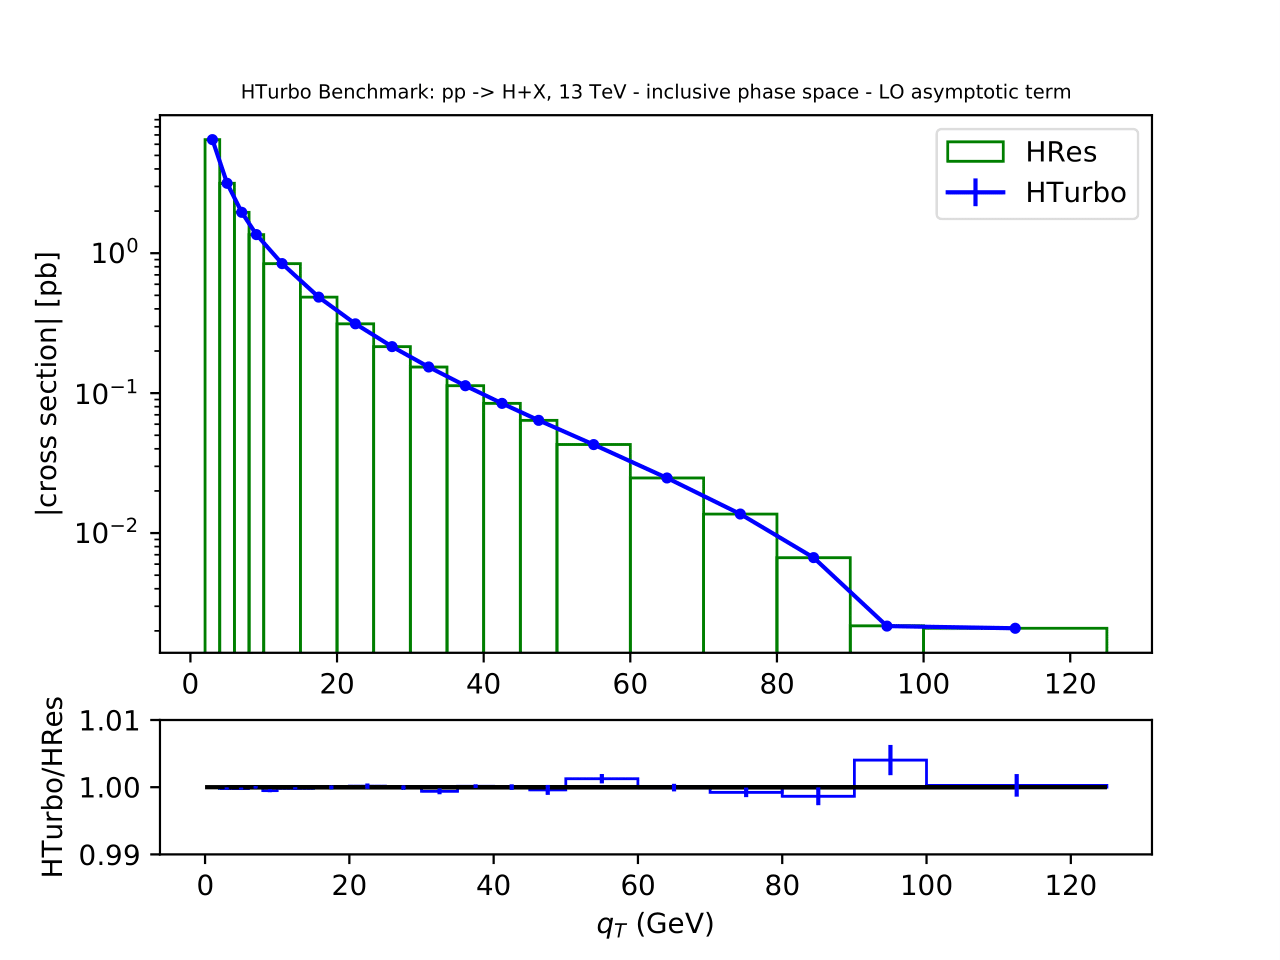
\includegraphics[width = 7cm]{plots/part3/chapter6/nlo-ct-1.png}
		\end{figure}
		
		\column{0.5\textwidth}
		
		\begin{figure}
			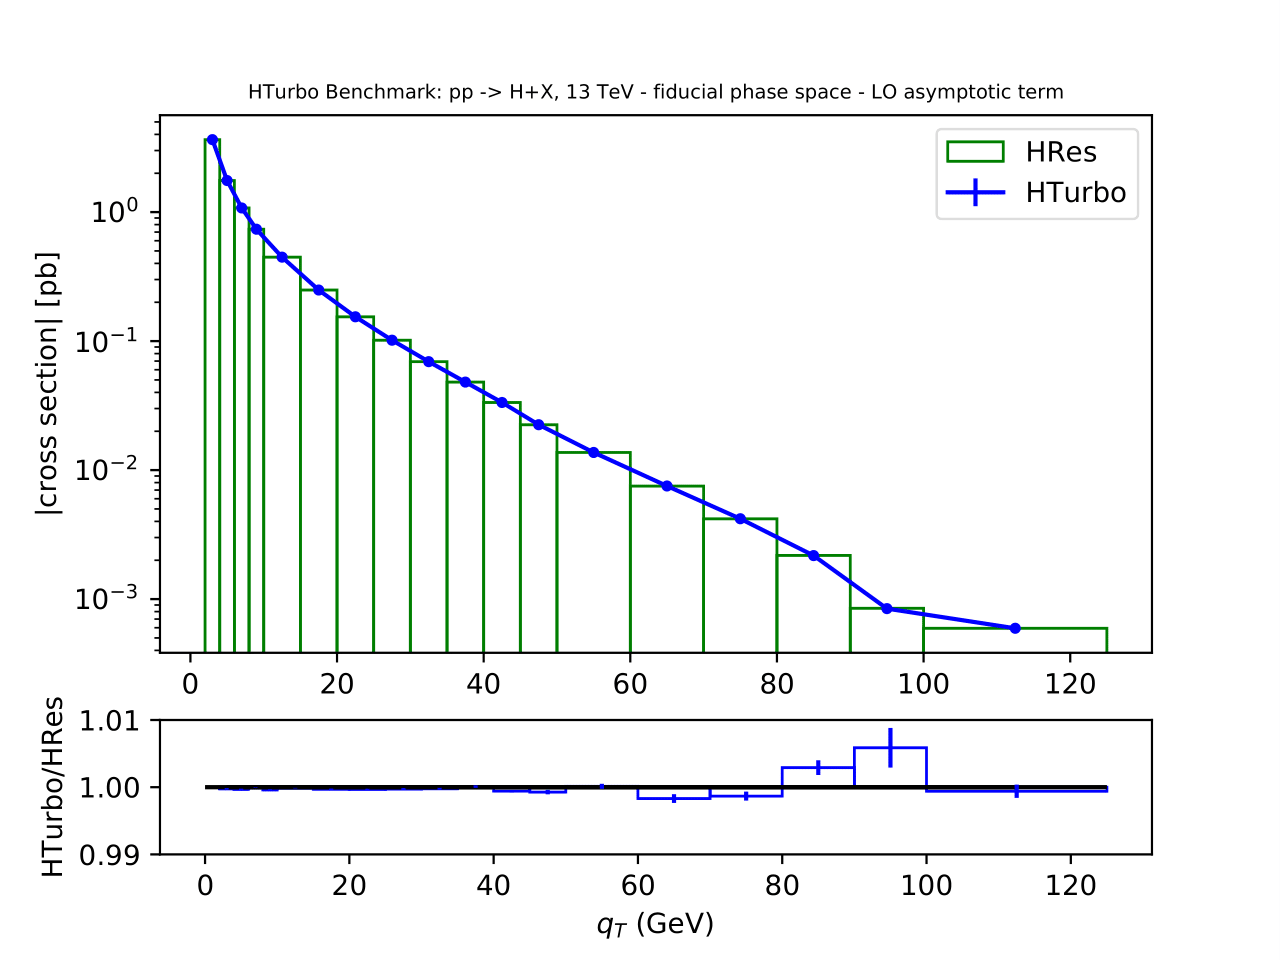
\includegraphics[width = 7cm]{plots/part3/chapter6/nlo-ct-fid-1.png}
		\end{figure}
		
	\end{columns}
	
	\begin{itemize}
		\item Cross section for fully inclusive (LHS) and fiducial (RHS) phase space {\color{darkgreen}$\checkmark$} 
		\item CM energy $\sqrt s = 13$ GeV and PDF set \texttt{NNPDF31\_nlo\_as\_0118 PDF} set
	\end{itemize}

\end{frame}

% Results - Benchmark HRes - NLO asymptotic
\begin{frame}
	
	\frametitle{Results}
	\framesubtitle{Comparison HTurbo and HRes - NLO asymptotic}

	\footnotesize
	
	\begin{columns}
		
		\column{0.5\textwidth}
		
		\begin{figure}
			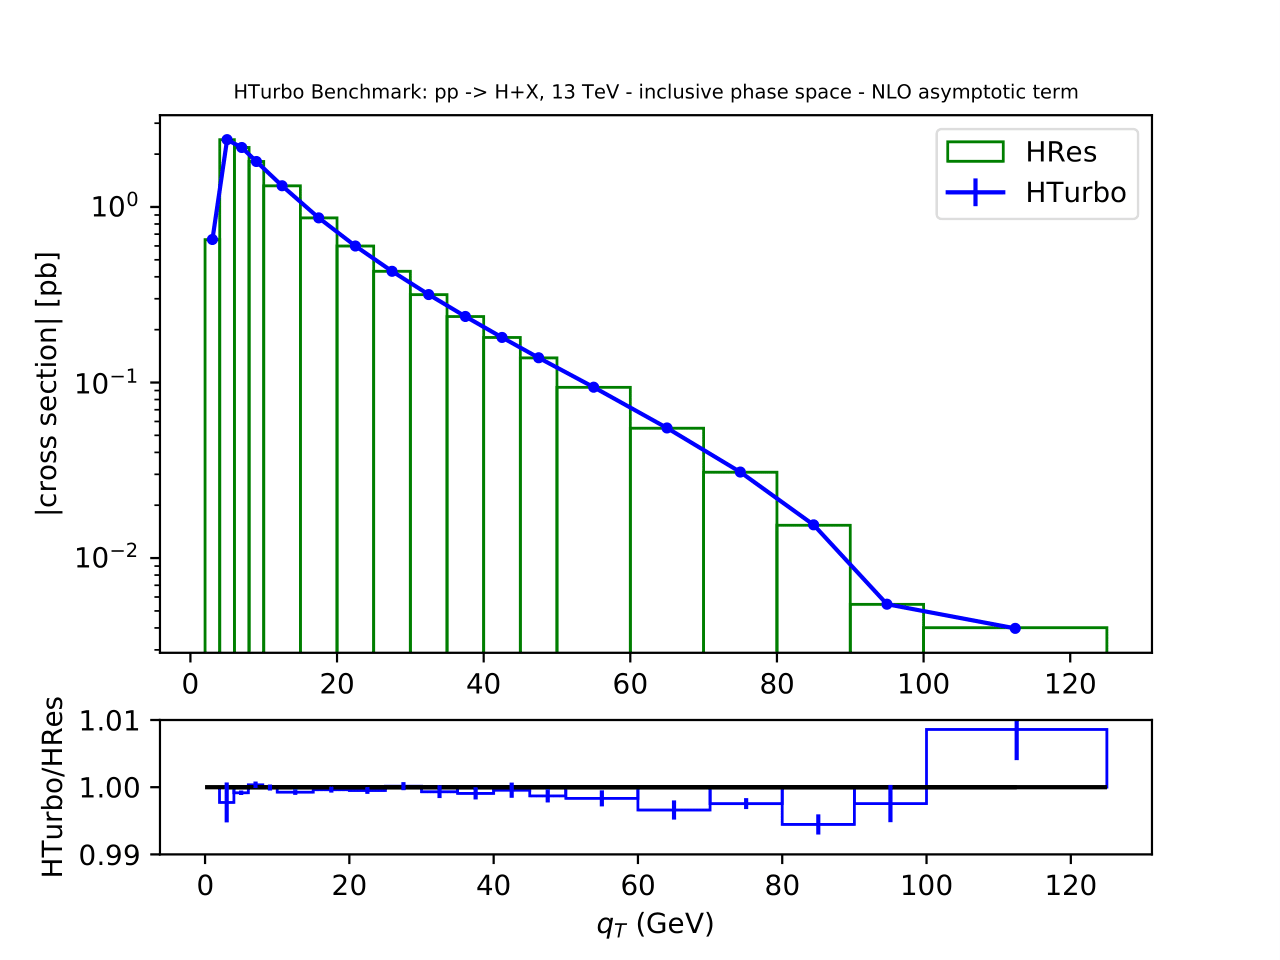
\includegraphics[width = 7cm]{plots/part3/chapter6/nnlo-ct-1.png}
		\end{figure}
		
		\column{0.5\textwidth}
		
		\begin{figure}
			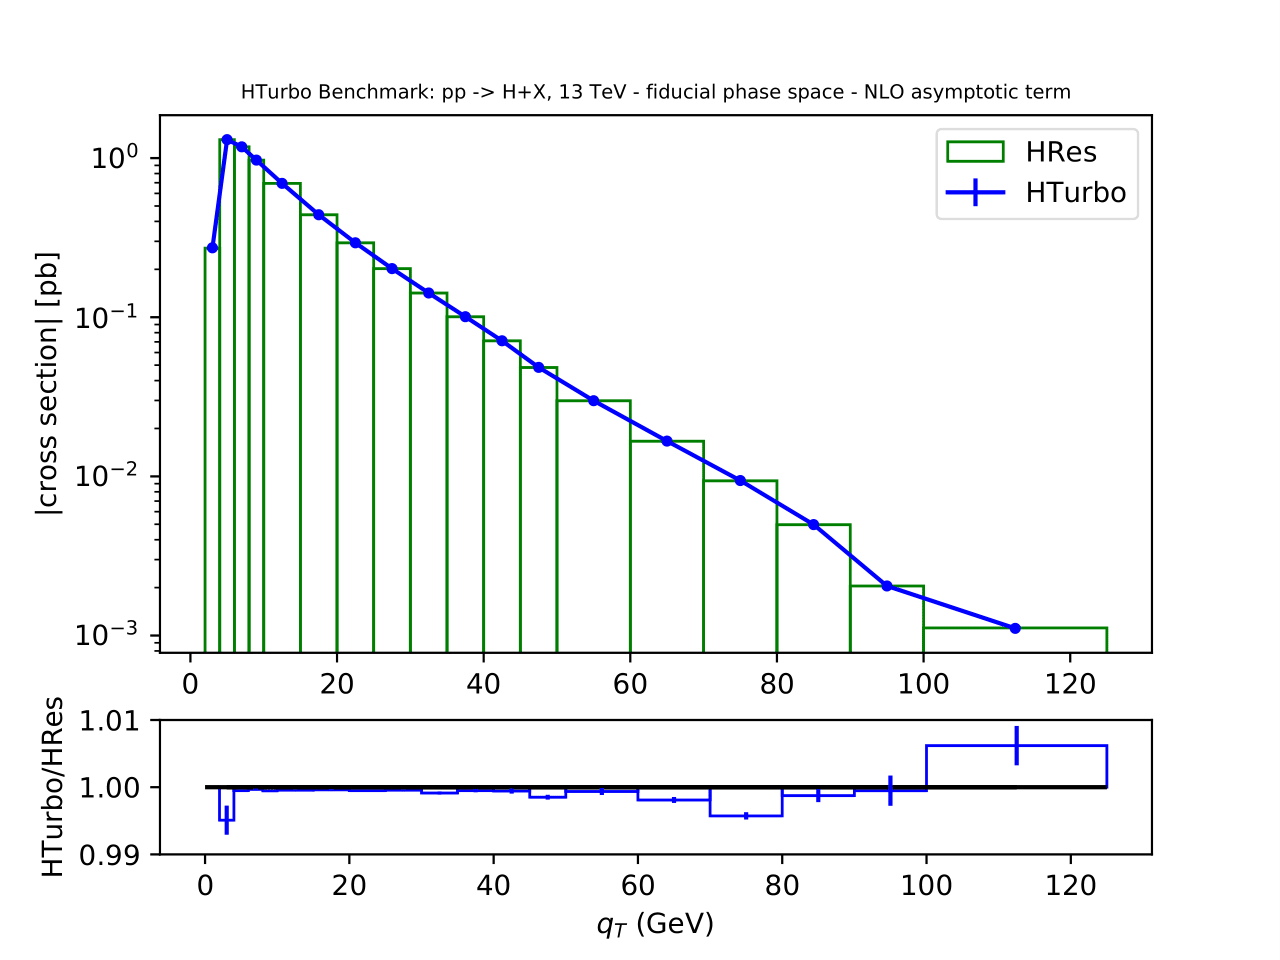
\includegraphics[width = 7cm]{plots/part3/chapter6/nnlo-ct-fid-1.png}
		\end{figure}
		
	\end{columns}
	
	\begin{itemize}
		\item Cross section for fully inclusive (LHS) and fiducial (RHS) phase space {\color{darkgreen}$\checkmark$} 
		\item CM energy $\sqrt s = 13$ GeV and PDF set \texttt{NNPDF31\_nnlo\_as\_0118 PDF} set
	\end{itemize}

\end{frame}

% Results - Benchmark HRes - LO fixed-order
\begin{frame}

	\frametitle{Results}
	\framesubtitle{Comparison HTurbo and HRes - LO fixed-order}
	
	\footnotesize
	
	\begin{columns}
		
		\column{0.5\textwidth}
		
		\begin{figure}
			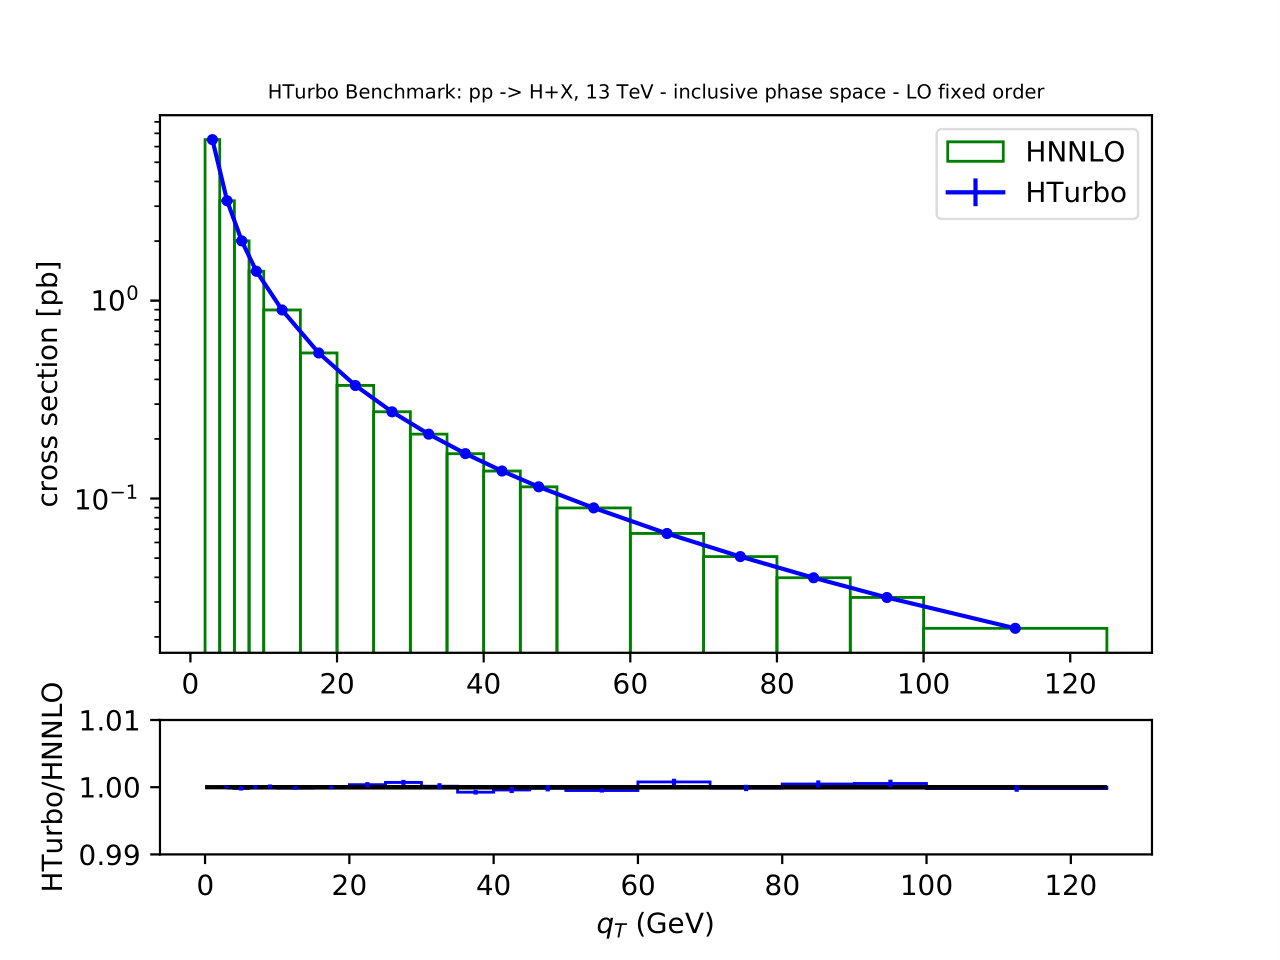
\includegraphics[width = 7cm]{plots/part3/chapter6/nlo-fo-1.png}
		\end{figure}
		
		\column{0.5\textwidth}
		
		\begin{figure}
			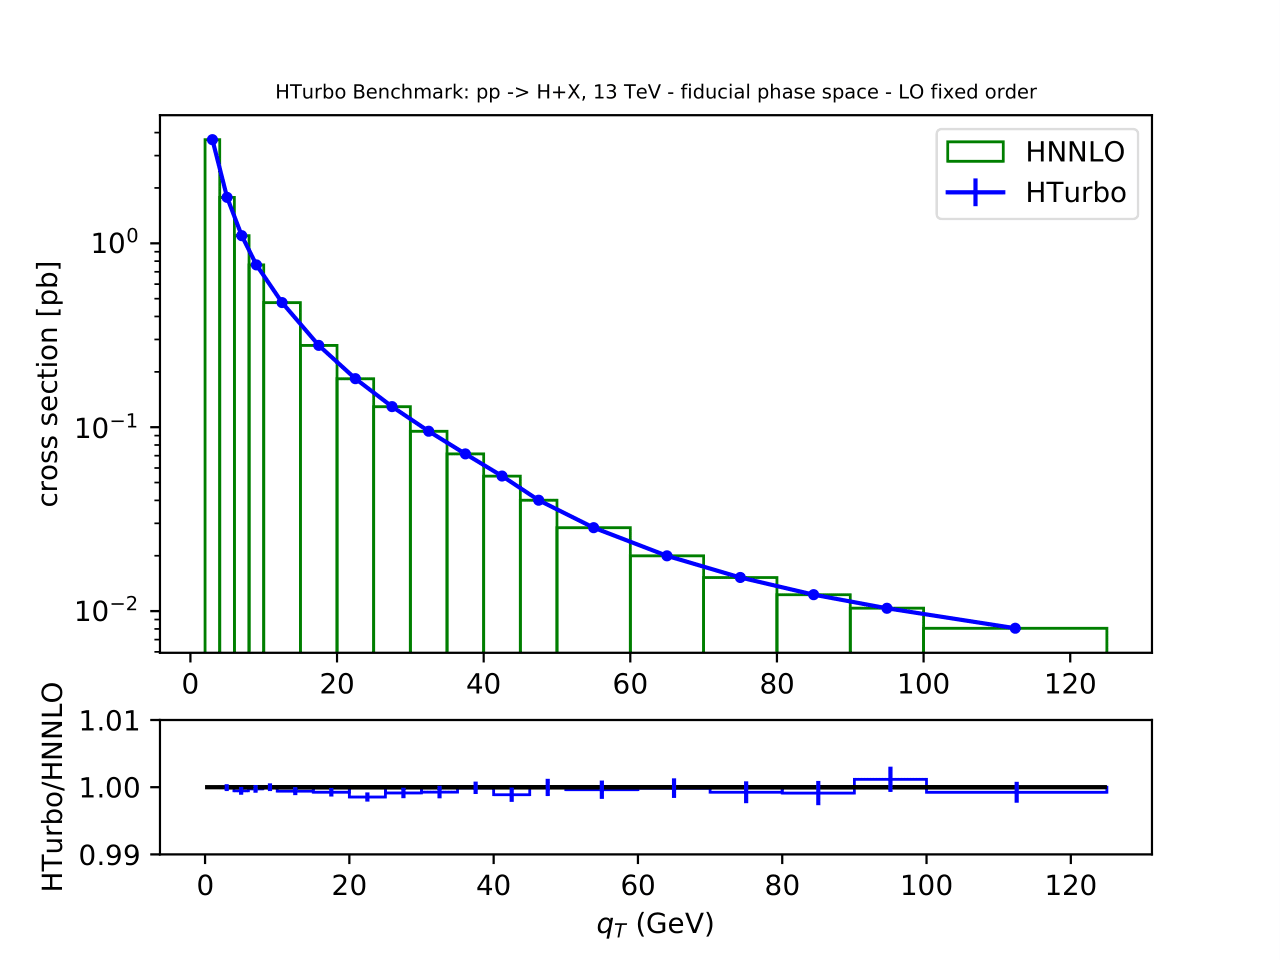
\includegraphics[width = 7cm]{plots/part3/chapter6/nlo-fo-fid-1.png}
		\end{figure}
		
	\end{columns}
	
	\begin{itemize}
		\item Cross section for fully inclusive (LHS) and fiducial (RHS) phase space {\color{darkgreen}$\checkmark$} 
		\item CM energy $\sqrt s = 13$ GeV and PDF set \texttt{NNPDF31\_nlo\_as\_0118 PDF} set
	\end{itemize}

\end{frame}

% Results - Benchmark HRes - LO fixed-order
\begin{frame}
	
	\frametitle{Results}
	\framesubtitle{Comparison HTurbo and HRes - NLO fixed-order}
	
	\footnotesize
	
	\begin{columns}
		
		\column{0.5\textwidth}
		
		\begin{figure}
			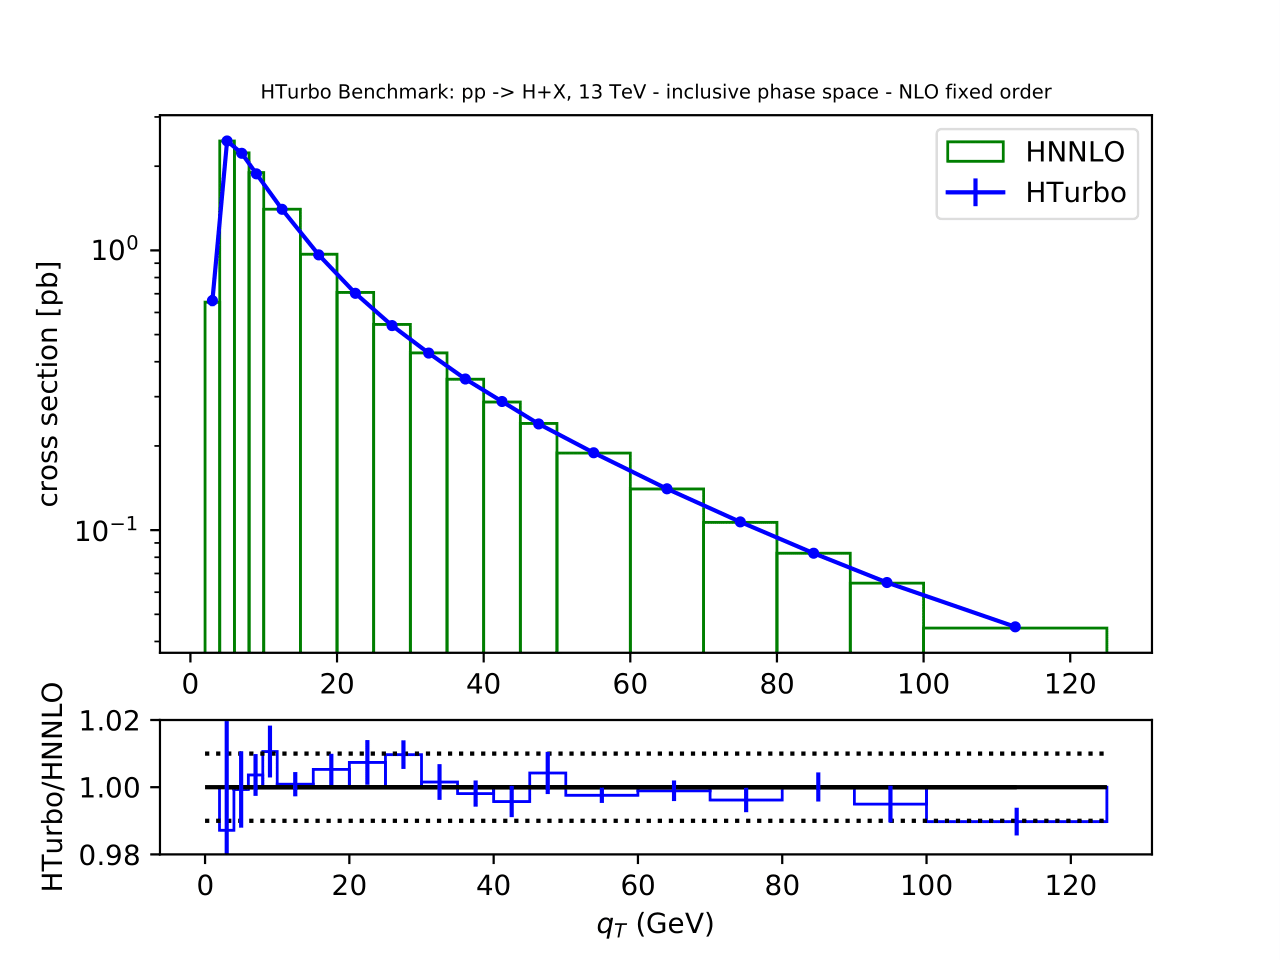
\includegraphics[width = 7cm]{plots/part3/chapter6/nnlo-fo-1.png}
		\end{figure}
		
		\column{0.5\textwidth}
		
		\begin{figure}
			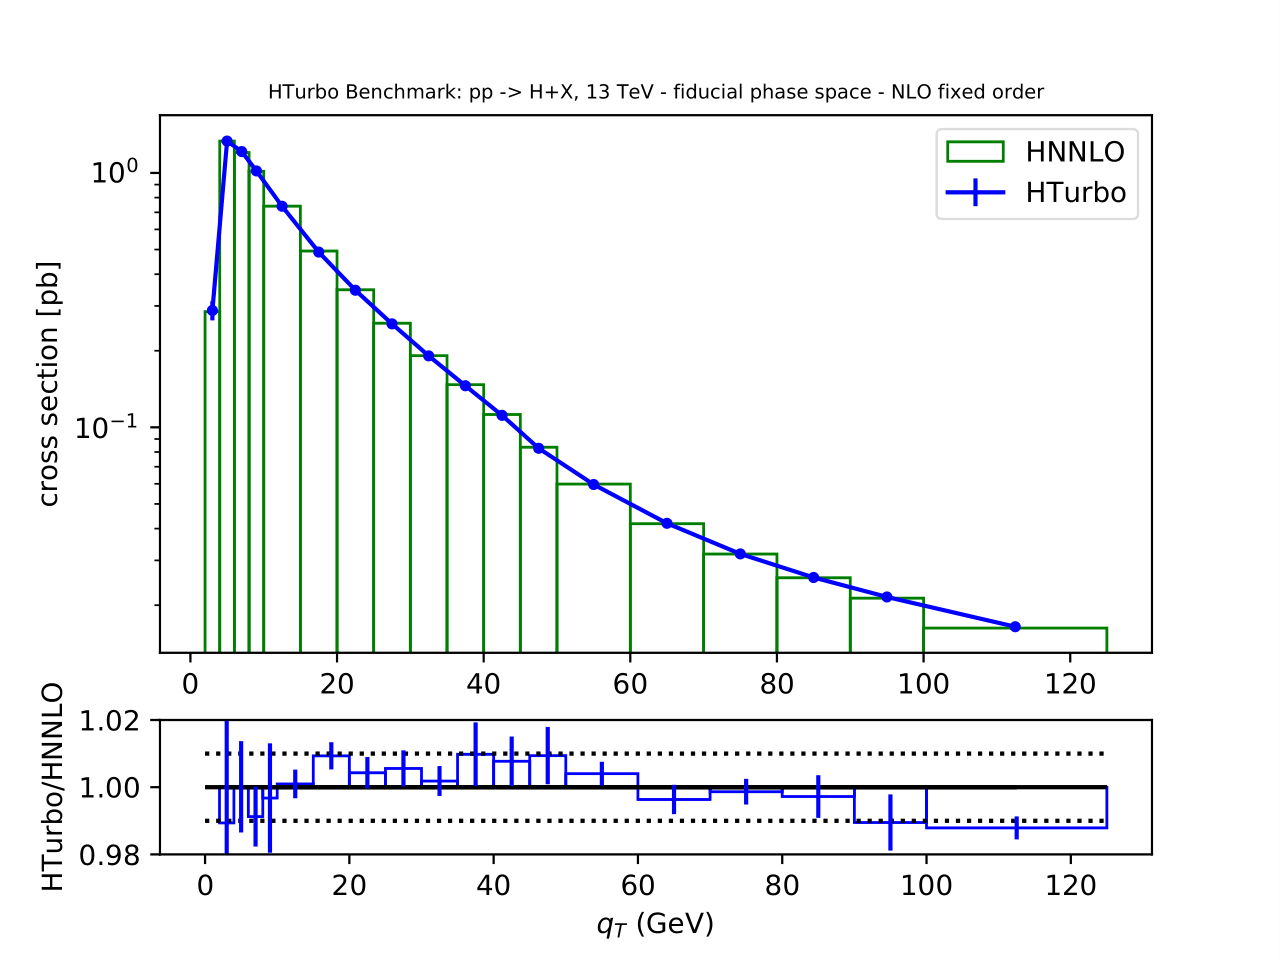
\includegraphics[width = 7cm]{plots/part3/chapter6/nnlo-fo-fid-1.png}
		\end{figure}
		
	\end{columns}
	
	\begin{itemize}
		\item Cross section for fully inclusive (LHS) and fiducial (RHS) phase space {\color{darkgreen}$\checkmark$} 
		\item CM energy $\sqrt s = 13$ GeV and PDF set \texttt{NNPDF31\_nnlo\_as\_0118 PDF} set
	\end{itemize}

\end{frame}

% Summary $\&$ Conclusions
\begin{frame}
	
	\frametitle{Summary $\&$ Conclusions}
	
	\vspace{2.0 cm}
	
	\begin{enumerate}
		\item \footnotesize Fast and accurate predictions are needed towards the precision era of the LHC
		\item \footnotesize Developing a novel numerical code, \textbf{HTurbo}, which implements $q_{\perp}$ resummation for Higgs boson production
		\item \footnotesize HTurbo is {\color{blue} faster than any of the existing codes}
		\item \footnotesize Outlook of thesis work: 
		\begin{itemize}
			\item \footnotesize Add {\color{blue}N$^{3}$LO+N$^{3}$LL} prediction
			\item \footnotesize Perform phenomenological studies comparing with LHC data
		\end{itemize}
		
	\end{enumerate}

	\vspace{2.0 cm}

\end{frame}

% Discussion $\&$ next steps
\begin{frame}
	
	\frametitle{Discussion $\&$ next steps}

	\vspace{2.0 cm}
	
	\begin{enumerate}
		\item \footnotesize Fast and accurate predictions are needed towards the precision era of the LHC
		\item \footnotesize Developing a novel numerical code, \textbf{HTurbo}, which implements $q_{\perp}$ resummation for Higgs boson production
		\item \footnotesize HTurbo is {\color{blue} faster than any of the existing codes}
		\item \footnotesize Outlook of thesis work: 
		\begin{itemize}
			\item \footnotesize Add {\color{blue}N$^{3}$LO+N$^{3}$LL} prediction
			\item \footnotesize Perform phenomenological studies comparing with LHC data
		\end{itemize}

	\end{enumerate}

	\vspace{2.0 cm}

\end{frame}

% Conclusions
\begin{frame}

	\center {\color{blue}Thank you!}

	\begin{figure}
		
\includegraphics[width = 2 cm]{plots/final/thinking.png}
	\end{figure}		

	{\small \color{blue} \footnotesize This project has received funding from the European Union$'$s Horizon 2020 research and innovation program under grant agreement No 740006.}

\end{frame}

% Back up
\begin{frame}

	\frametitle{Back up}

\end{frame}

% Back up
\begin{frame}

	\frametitle{Back up}

\end{frame}

% Back up
\begin{frame}

	\frametitle{Back up}

\end{frame}

\end{document}
